%------------------------------------------------------------------------------%
% setup documentclass

% EN: This file is loaded before the \documentclass command in the main document

% EN: The following package allows \\ at the title page
%     For more information see https://github.com/latextemplates/scientific-thesis-cover/issues/4
\RequirePackage{kvoptions-patch}

\ifenglisch
  \PassOptionsToClass{numbers=noenddot}{scrbook}
\else
  %()Aus scrguide.pdf - der Dokumentation von KOMA-Script)
  %Nach DUDEN steht in Gliederungen, in denen ausschließlich arabische Ziffern für die Nummerierung
  %verwendet werden, am Ende der Gliederungsnummern kein abschließender Punkt
  %(siehe [DUD96, R3]). Wird hingegen innerhalb der Gliederung auch mit römischen Zahlen
  %oder Groß- oder Kleinbuchstaben gearbeitet, so steht am Ende aller Gliederungsnummern ein
  %abschließender Punkt (siehe [DUD96, R4])
  \PassOptionsToClass{numbers=autoendperiod}{scrbook}
\fi

% Warns about outdated packages and missing caption declarations
% See https://www.ctan.org/pkg/nag
\RequirePackage[l2tabu, orthodox]{nag}

%DE: Neue deutsche Trennmuster
%    Siehe http://www.ctan.org/pkg/dehyph-exptl und http://projekte.dante.de/Trennmuster/WebHome
%    Nur für pdflatex, nicht für lualatex
\RequirePackage{ifluatex}
\ifluatex
  % do not load anything
\else
  \ifdeutsch
    \RequirePackage[ngerman=ngerman-x-latest]{hyphsubst}
  \fi
\fi


\documentclass[%
    % fontsize=11pt is the standard
    a4paper,  % Standard format - only KOMAScript uses paper=a4 - https://tex.stackexchange.com/a/61044/9075
    twoside,  % we are optimizing for both screen and two-side printing. So the page numbers will jump, but the content is configured to stay in the middle (by using the geometry package)
    bibliography=totoc,
    %               idxtotoc,   %Index ins Inhaltsverzeichnis
    %               liststotoc, %List of X ins Inhaltsverzeichnis, mit liststotocnumbered werden die Abbildungsverzeichnisse nummeriert
    headsepline,
    cleardoublepage=empty,
    parskip=half,
    %               draft    % um zu sehen, wo noch nachgebessert werden muss - wichtig, da Bindungskorrektur mit drin
    draft=false
]{scrbook}
% EN: This file includes basic packages and sets options. The order of package
%     loading is important

% DE: In dieser Datei werden zuerst die benoetigten Pakete eingebunden und
%     danach diverse Optionen gesetzt. Achtung Reihenfolge ist entscheidend!


% EN: Styleguide:
% - English comments are prefixed with "EN", German comments are prefixed with "DE"
% - Prefixed headings define the language for the subsequent paragraphs
% - It is tried to organize packages in blocks. Bocks are separated by two empty lines.

% DE: Styleguide:
%
% Ein sehr kleiner Styleguide. Packages werden in Blöcken organisiert.
% Zwischen zwei Blöcken sind 2 Leerzeilen!


% EN: Enable copy and paste of text from the PDF
%     Only required for pdflatex. It "just works" in the case of lualatex.
%     mmap enables mathematical symbols, but does not work with the newtx font set
%     See: https://tex.stackexchange.com/a/64457/9075
%     Other solutions outlined at http://goemonx.blogspot.de/2012/01/pdflatex-ligaturen-und-copynpaste.html and http://tex.stackexchange.com/questions/4397/make-ligatures-in-linux-libertine-copyable-and-searchable
%     Trouble shooting outlined at https://tex.stackexchange.com/a/100618/9075

\ifluatex
\else
  \usepackage{cmap}
\fi


% EN: File encoding
% DE: Codierung
%     Wir sind im 21 Jahrhundert, utf-8 löst so viele Probleme.
%
% Mit UTF-8 funktionieren folgende Pakete nicht mehr. Bitte beachten!
%   * fancyvrb mit §
%   * easylist -> http://www.ctan.org/tex-archive/macros/latex/contrib/easylist/
\ifluatex
  % EN: See https://tex.stackexchange.com/a/158517/9075
  %     Not required, because of usage of fontspec package
  %\usepackage[utf8]{luainputenc}
\else
  \usepackage[utf8]{inputenc}
\fi


% DE: Parallelbetrieb tex4ht und pdflatex

\makeatletter
\@ifpackageloaded{tex4ht}{
  \def\iftex4ht{\iftrue}
}{
  \def\iftex4ht{\iffalse}
}
\makeatother


% EN: Mathematics
% DE: Mathematik
%
% DE: Viele Mathematik-Sachen. Siehe https://texdoc.net/pkg/amsmath
%
% EN: Options must be passed this way, otherwise it does not work with glossaries
% DE: fleqn (=Gleichungen linksbündig platzieren) funktioniert nicht direkt. Es muss noch ein Patch gemacht werden:
\PassOptionsToPackage{fleqn,leqno}{amsmath}
%
% DE: amsmath Muss nicht mehr geladen werden, da es von newtxmath automatisch geladen wird
% \usepackage{amsmath}


%% EN: Fonts
%% DE: Schriften
%%
%% !!! If you change the font, be sure that words such as "workflow" can
%% !!! still be copied from the PDF. If this is not the case, you have
%% !!! to use glyphtounicode. See comment at cmap package


% EN: Times Roman for all text
\ifluatex
  % source: Second proposed fix from the following answer: https://tex.stackexchange.com/a/394137
  \usepackage[no-math]{fontspec}
  \setmainfont{TeXGyreTermes-Regular}[
       BoldFont       = TeXGyreTermes-Bold ,
       ItalicFont     = TeXGyreTermes-Italic ,
       BoldItalicFont = TeXGyreTermes-BoldItalic,
       NFSSFamily     = ntxtlf]
  \setsansfont{TeX Gyre Heros Regular}[
       Scale=.9,
       BoldFont       = TeX Gyre Heros Bold,
       ItalicFont     = TeX Gyre Heros Italic,
       BoldItalicFont = TeX Gyre Heros BoldItalic]
  \setmonofont[StylisticSet={1,3},Scale=.9]{inconsolata}
  \RequirePackage{newtxmath}
\else
  \RequirePackage{newtxtext}
  \RequirePackage{newtxmath}
  % EN: looks good with times, but no equivalent for lualatex found,
  %     therefore replaced with inconsolata
  %\RequirePackage[zerostyle=b,scaled=.9]{newtxtt}
  \RequirePackage[varl,scaled=.9]{inconsolata}
\fi

% EN: Fallback font - if the subsequent font packages do not define a font (e.g., monospaced)
%     This is the modern package for "Computer Modern".
%     In case this gets activated, one has to switch from cmap package to glyphtounicode (in the case of pdflatex)
% DE: Fallback-Schriftart
%\usepackage[%
%    rm={oldstyle=false,proportional=true},%
%    sf={oldstyle=false,proportional=true},%
%    tt={oldstyle=false,proportional=true,variable=true},%
%    qt=false%
%]{cfr-lm}

% EN: Headings are typset in Helvetica (which is similar to Arial)
% DE: Schriftart fuer die Ueberschriften - ueberschreibt lmodern
%\usepackage[scaled=.95]{helvet}

% DE: Für Schreibschrift würde tun, muss aber nicht
%\usepackage{mathrsfs} %  \mathscr{ABC}

% EN: Font for the main text
% DE: Schriftart fuer den Fliesstext - ueberschreibt lmodern
%     Linux Libertine, siehe http://www.linuxlibertine.org/
%     Packageparamter [osf] = Minuskel-Ziffern
%     rm = libertine im Brottext, Linux Biolinum NICHT als serifenlose Schrift, sondern helvet (von oben) beibehalten
%\usepackage[rm]{libertine}

% EN: Alternative Font: Palantino. It is recommeded by Prof. Ludewig for German texts
% DE: Alternative Schriftart: Palantino, Packageparamter [osf] = Minuskel-Ziffern
%     Bitte nur in deutschen Texten
%\usepackage{mathpazo} %ftp://ftp.dante.de/tex-archive/fonts/mathpazo/ - Tipp aus DE-TEX-FAQ 8.2.1

% DE: Schriftart fuer Programmcode - ueberschreibt lmodern
%     Falls auskommentiert, wird die Standardschriftart lmodern genommen
%     Fuer schreibmaschinenartige Schluesselwoerter in den Listings - geht bei alten Installationen nicht, da einige Fontshapes (<>=) fehlen
%\usepackage[scaled=.92]{luximono}
%\usepackage{courier}
% DE: BeraMono als Typewriter-Schrift, Tipp von http://tex.stackexchange.com/a/71346/9075
%\usepackage[scaled=0.83]{beramono}

% EN: backticks (`) are rendered as such in verbatim environments.
%     See following links for details:
%     - https://tex.stackexchange.com/a/341057/9075
%     - https://tex.stackexchange.com/a/47451/9075
%     - https://tex.stackexchange.com/a/166791/9075
\usepackage{upquote}

% DE: Symbole
%
%\usepackage[geometry]{ifsym} % \BigSquare
%\usepackage{mathabx}
%\usepackage{stmaryrd} %fuer \ovee, \owedge, \otimes
%\usepackage{marvosym} %fuer \Writinghand %patched to not redefine \Rightarrow
%\usepackage{mathrsfs} %mittels \mathscr{} schoenen geschwungenen Buchstaben erzeugen
%\usepackage{calrsfs} %\mathcal{} ein bisserl dickeren buchstaben erzeugen - sieht net so gut aus.
%durch mathpazo ist das schon definiert

%
%\usepackage{amssymb}

% EN: For \texttrademark{}
\usepackage{textcomp}

% EN: name-clashes von marvosym und mathabx vermeiden:
\def\delsym#1{%
  %  \expandafter\let\expandafter\origsym\expandafter=\csname#1\endcsname
  %  \expandafter\let\csname orig#1\endcsname=\origsym
  \expandafter\let\csname#1\endcsname=\relax
}

%\usepackage{pifont}
%\usepackage{bbding}
%\delsym{Asterisk}
%\delsym{Sun}\delsym{Mercury}\delsym{Venus}\delsym{Earth}\delsym{Mars}
%\delsym{Jupiter}\delsym{Saturn}\delsym{Uranus}\delsym{Neptune}
%\delsym{Pluto}\delsym{Aries}\delsym{Taurus}\delsym{Gemini}
%\delsym{Rightarrow}
%\usepackage{mathabx} - Ueberschreibt leider zu viel - und die \le-Zeichen usw. sehen nicht gut aus!


% EN: Modern font encoding
%     Has to be loaded AFTER any font packages. See https://tex.stackexchange.com/a/2869/9075.
\ifluatex
\else
  \usepackage[T1]{fontenc}
\fi
%


% EN: Character protrusion and font expansion. See http://www.ctan.org/tex-archive/macros/latex/contrib/microtype/
% DE: Optischer Randausgleich und Grauwertkorrektur

\usepackage[
  babel=true, % EN: Enable language-specific kerning. Take language-settings from the languge of the current document (see Section 6 of microtype.pdf)
  expansion=alltext,
  protrusion=alltext-nott, % EN: Ensure that at listings, there is no change at the margin of the listing
  final % EN: Always enable microtype, even if in draft mode. This helps finding bad boxes quickly.
        %     In the standard configuration, this template is always in the final mode, so this option only makes a difference if "pros" use the draft mode
]{microtype}


% EN: \texttt{test -- test} keeps the "--" as "--" (and does not convert it to an en dash)
\DisableLigatures{encoding = T1, family = tt* }

% DE: fuer microtype
% DE: tracking=true muss als Parameter des microtype-packages mitgegeben werden
% DE: Deaktiviert, da dies bei Algorithmen seltsam aussieht

%\DeclareMicrotypeSet*[tracking]{my}{ font = */*/*/sc/* }%
%\SetTracking{ encoding = *, shape = sc }{ 45 }
% DE: Hier wird festgelegt,
%     dass alle Passagen in Kapitälchen automatisch leicht
%     gesperrt werden.
%     Quelle: http://homepage.ruhr-uni-bochum.de/Georg.Verweyen/pakete.html
%    Deaktiviert, da sonst "BPEL", "BPMN" usw. wirklich komisch aussehen.
%     Macht wohl nur bei geisteswissenschaftlichen Arbeiten Sinn.


% EN: amsmath teaks


% EN: Fixes bugs in AMS math
%     Corrently conflicts with unicode-math
% \usepackage{mathtools}

%\numberwithin{equation}{section}
%\renewcommand{\theequation}{\thesection.\Roman{equation}}

% EN: work-around ams-math problem with align and 9 -> 10. Does not work with glossaries, No visual changes.
%\addtolength\mathindent{1em}


% EN: For theorems, replacement for amsthm
\usepackage[amsmath,hyperref]{ntheorem}
\theorempreskipamount 2ex plus1ex minus0.5ex
\theorempostskipamount 2ex plus1ex minus0.5ex
\theoremstyle{break}
\newtheorem{definition}{Definition}[section]


% CTAN: https://ctan.org/pkg/lccaps
% Doc: http://texdoc.net/pkg/lccaps
%
% Required for DE/EN \initialism
\usepackage{lccaps}


% EN: Defintion of colors. Argument "hyperref" is not used as we do not want to change border colors of links: Links are not colored anymore.
% DE: Farbdefinitionen
\usepackage[dvipsnames]{xcolor}


% EN: Required for custom acronyms/glossaries style.
%     Left aligned Columns in tables with fixed width.
%     See http://tex.stackexchange.com/questions/91566/syntax-similar-to-centering-for-right-and-left
\usepackage{ragged2e}


% DE: Wichtig, ansonsten erscheint "No room for a new \write"
\usepackage{scrwfile}


% EN: Support for language-specific hyphenation
% DE: Neue deutsche Rechtschreibung und Literatur statt "Literature"
%     Die folgende Einstellung ist der Nachfolger von ngerman.sty
\ifenglish
  % EN: Set English as language and allow to write hyphenated"=words
  %     `american`, `english` and `USenglish` are synonyms for babel package (according to https://tex.stackexchange.com/questions/12775/babel-english-american-usenglish).
  %      "english" has to go last to set it as default language
  \usepackage[ngerman,main=english]{babel}
  % EN: Hint by http://tex.stackexchange.com/a/321066/9075 -> enable "= as dashes
  \addto\extrasenglish{\languageshorthands{ngerman}\useshorthands{"}}
  \ifluatex
    % EN: conditionally disable ligatures. See https://github.com/latextemplates/scientific-thesis-template/issues/54
    %     for a discussion
    \usepackage[english]{selnolig}
  \fi
\fi
\ifdeutsch
  % DE: letzte Sprache ist default, Einbindung von "american" ermöglicht \begin{otherlanguage}{amercian}...\end{otherlanguage} oder \foreignlanguage{american}{Text in American}
  %     Siehe auch http://tex.stackexchange.com/a/50638/9075
  \usepackage[american,main=ngerman]{babel}
  % Ein "abstract" ist eine "Kurzfassung", keine "Zusammenfassung"
  \addto\captionsngerman{%
    \renewcommand\abstractname{Kurzfassung}%
  }
  \ifluatex
    % EN: conditionally disable ligatures. See https://github.com/latextemplates/scientific-thesis-template/issues/54
    %     for a discussion
    \usepackage[ngerman]{selnolig}
  \fi
\fi
%


% EN: For easy quotations: \enquote{text}
%     This package is very smart when nesting is applied, otherwise textcmds (see below) provides a shorter command
%     Note that this package results in a warning when it is loaded before minted (actually fvextra).
% DE: Anführungszeichen
%     Zitate in \enquote{...} setzen, dann werden automatisch die richtigen Anführungszeichen verwendet.
%     Dieses package erzeugt eine Warnung, wenn es vor minted (genauer fvextra) geladen wird.
\usepackage{csquotes}


% EN: For even easier quotations: \qq{text}.
%     Is not smart in the case of nesting, but good enough for the most cases
\usepackage{textcmds}
\ifdeutsch
  % EN: German quotes are different. So do not use the English quotes, but the ones provided by the csquotes package.
  \renewcommand{\qq}[1]{\enquote{#1}}
\fi


% EN: extended enumarations
% DE: erweitertes Enumerate
\usepackage{paralist}


% DE: Gestaltung der Kopf- und Fußteilen

\usepackage[automark]{scrlayer-scrpage}

\automark[section]{chapter}
\setkomafont{pageheadfoot}{\normalfont\sffamily}
\setkomafont{pagenumber}{\normalfont\sffamily}

% DE: funktioniert nicht: Alle Linien sind hier weg
%\setheadsepline[.4pt]{.4pt}


% DE: Intelligentes Leerzeichen um hinter Abkürzungen die richtigen Abstände zu erhalten, auch leere.
%     Siehe commands.tex \gq{}
\usepackage{xspace}
% DE: Macht \xspace und \enquote kompatibel
\makeatletter
\xspaceaddexceptions{\grqq \grq \csq@qclose@i \} }
\makeatother


\newcommand{\eg}{e.\,g.,\ }
\newcommand{\ie}{i.\,e.,\ }


% EN: introduce \powerset - hint by http://matheplanet.com/matheplanet/nuke/html/viewtopic.php?topic=136492&post_id=997377
\DeclareFontFamily{U}{MnSymbolC}{}
\DeclareSymbolFont{MnSyC}{U}{MnSymbolC}{m}{n}
\DeclareFontShape{U}{MnSymbolC}{m}{n}{
  <-6>    MnSymbolC5
  <6-7>   MnSymbolC6
  <7-8>   MnSymbolC7
  <8-9>   MnSymbolC8
  <9-10>  MnSymbolC9
  <10-12> MnSymbolC10
  <12->   MnSymbolC12%
}{}
\DeclareMathSymbol{\powerset}{\mathord}{MnSyC}{180}


% EN: Package for the appendix
% DE: Anhang
\usepackage{appendix}
%[toc,page,title,header]
%


% EN: Graphics
% DE: Grafikeinbindungen
%
% EN: The parameter "pdftex" is not required
\usepackage{graphicx}
\graphicspath{{\getgraphicspath}}
\newcommand{\getgraphicspath}{res/graphics/}


% EN: Enables inclusion of SVG graphics - 1:1 approach
%    This is NOT the approach of https://ctan.org/pkg/svg-inkscape,
%     which allows text in SVG to be typeset using LaTeX
%     We just include the SVG as is.
\usepackage{epstopdf}
\epstopdfDeclareGraphicsRule{.svg}{pdf}{.pdf}{%
  inkscape -z -D --file=#1 --export-pdf=\OutputFile
}


% EN: Enables inclusion of SVG graphics - text-rendered-with-LaTeX-approach
%     This is the approach of https://ctan.org/pkg/svg-inkscape,
\newcommand{\executeiffilenewer}[3]{%
  \IfFileExists{#2}
  {
    %\message{file #2 exists}
    \ifnum\pdfstrcmp{\pdffilemoddate{#1}}%
      {\pdffilemoddate{#2}}>0%
      {\immediate\write18{#3}}
    \else
      {%\message{file up to date #2}
      }
    \fi%
  }{
    %\message{file #2 doesn't exist}
    %\message{argument: #3}
    %\immediate\write18{echo "test" > xoutput.txt}
    \immediate\write18{#3}
  }
}
\newcommand{\includesvg}[1]{%
  \executeiffilenewer{#1.svg}{#1.pdf}%
  {
    inkscape -z -D --file=\getgraphicspath#1.svg %
    --export-pdf=\getgraphicspath#1.pdf --export-latex}%
  \input{\getgraphicspath#1.pdf_tex}%
}


% EN: Enable typesetting values with SI units.
\ifenglish
  \usepackage[mode=text,group-four-digits,group-separator={,}]{siunitx}
  \sisetup{locale=US}
\fi
\ifdeutsch
  \usepackage[mode=text,group-four-digits]{siunitx}
  \sisetup{locale=DE}
\fi


% EN: Extensions for tables
% DE: Tabellenerweiterungen
\usepackage{array} %increases tex's buffer size and enables ``>'' in tablespecs
\usepackage{longtable}
\usepackage{dcolumn} %Aligning numbers by decimal points in table columns
\ifenglish
  \newcolumntype{d}[1]{D{.}{.}{#1}}
\fi
\ifdeutsch
  \newcolumntype{d}[1]{D{.}{,}{#1}}
\fi
\setlength{\extrarowheight}{1pt}


% DE: Eine Zelle, die sich über mehrere Zeilen erstreckt.
%     Siehe Beispieltabelle in Kapitel 2
\usepackage{multirow}


% DE: Fuer Tabellen mit Variablen Spaltenbreiten
%\usepackage{tabularx}
%\usepackage{tabulary}


% EN: Links behave as they should. Enables "\url{...}" for URL typesettings.
%     Allow URL breaks also at a hyphen, even though it might be confusing: Is the "-" part of the address or just a hyphen?
%     See https://tex.stackexchange.com/a/3034/9075.
% DE: Links verhalten sich so, wie sie sollen
%     Zeilenumbrüche bei URLs auch bei Bindestrichen erlauben, auch wenn es verwirrend sein könnte: Gehört der Bindestrich zur URL oder ist es ein Trennstrich?
%     Siehe https://tex.stackexchange.com/a/3034/9075.
\usepackage[hyphens]{url}
%
%  EN: When activated, use text font as url font, not the monospaced one.
%      For all options see https://tex.stackexchange.com/a/261435/9075.
% \urlstyle{same}
%
% EN: Hint by http://tex.stackexchange.com/a/10419/9075.
\makeatletter
\g@addto@macro{\UrlBreaks}{\UrlOrds}
\makeatother


% DE: Index über Begriffe, Abkürzungen
%\usepackage{makeidx} makeidx ist out -> http://xindy.sf.net verwenden


% DE: lustiger Hack fuer das Abkuerzungsverzeichnis
%     nach latex durchlauf folgendes ausfuehren
%     makeindex ausarbeitung.nlo -s nomencl.ist -o ausarbeitung.nls
%     danach nochmal latex
%\usepackage{nomencl}
%    \let\abk\nomenclature %Deutsche Ueberschrift setzen
%          \renewcommand{\nomname}{List of Abbreviations}
%        %Punkte zw. Abkuerzung und Erklaerung
%          \setlength{\nomlabelwidth}{.2\hsize}
%          \renewcommand{\nomlabel}[1]{#1 \dotfill}
%        %Zeilenabstaende verkleinern
%          \setlength{\nomitemsep}{-\parsep}
%    \makenomenclature


% EN: Logic for TeX - enables if-then-else in commands
% DE: Logik für TeX
%     FÜr if-then-else @ commands.tex
\usepackage{ifthen}


% EN: Code Listings
% DE: Listings
\usepackage{listings}
\lstset{language=XML,
  showstringspaces=false,
  extendedchars=true,
  basicstyle=\footnotesize\ttfamily,
  commentstyle=\slshape,
  % DE: Original: \rmfamily, damit werden die Strings im Quellcode hervorgehoben. Zusaetzlich evtl.: \scshape oder \rmfamily durch \ttfamily ersetzen. Dann sieht's aus, wie bei fancyvrb
  stringstyle=\ttfamily,
  breaklines=true,
  breakatwhitespace=true,
  % EN: alternative: fixed
  columns=flexible,
  numbers=left,
  numberstyle=\tiny,
  basewidth=.5em,
  xleftmargin=.5cm,
  % aboveskip=0mm, %DE: deaktivieren, falls man lstlistings direkt als floating object benutzt (\begin{lstlisting}[float,...])
  % belowskip=0mm, %DE: deaktivieren, falls man lstlistings direkt als floating object benutzt (\begin{lstlisting}[float,...])
  captionpos=b
}

\ifluatex
\else
  % EN: Enable UTF-8 support - see https://tex.stackexchange.com/q/419327/9075
  \usepackage{listingsutf8}
  \lstset{inputencoding=utf8/latin1}
\fi

\ifdeutsch
  \renewcommand{\lstlistlistingname}{Verzeichnis der Listings}
\fi


% EN: Alternative to listings could be fancyvrb. Can be used together.
% DE: Alternative zu Listings ist fancyvrb. Kann auch beides gleichzeitig benutzt werden.
\usepackage{fancyvrb}
%
% EN: Font size for the normal text
% DE: Groesse fuer den Fliesstext. Falls deaktiviert: \normalsize
%\fvset{fontsize=\small}
%
% DE: Somit kann im Text ganz einfach §verbatim§ text gesetzt werden.
%     Disabled, because UTF-8 does not work any more and lualatex causes issues
%\DefineShortVerb{\§}
%
% EN: Shrink font size of listings
\RecustomVerbatimEnvironment{Verbatim}{Verbatim}{fontsize=\footnotesize}
\RecustomVerbatimCommand{\VerbatimInput}{VerbatimInput}{fontsize=\footnotesize}
%
% EN: Hack for fancyvrb based on http://newsgroups.derkeiler.com/Archive/Comp/comp.text.tex/2008-12/msg00075.html
%     Change of the solution: \Vref somehow collidated with cleveref/varioref as the output of \Vref{} was "Abschnitt 4.3 auf Seite 85"; therefore changed to \myVref -- so completely removed
%     See https://tex.stackexchange.com/q/132420/9075 for more information.
\newcommand{\Vlabel}[1]{\label[line]{#1}\hypertarget{#1}{}}
\newcommand{\lref}[1]{\hyperlink{#1}{\FancyVerbLineautorefname~\ref*{#1}}}


% EN: Tunings of captions for floats, listings, ...
% DE: Bildunterschriften bei floats genauso formatieren wie bei Listings
%     Anpassung wird unten bei den newfloat-Deklarationen vorgenommen
%     https://www.ctan.org/pkg/caption2 is superseeded by this package.
\usepackage{caption}


% EN: Provides rotating figures, where the PDF page is also turned
% DE: Ermoeglicht es, Abbildungen um 90 Grad zu drehen
%     Alternatives Paket: rotating Allerdings wird hier nur das Bild gedreht, während bei lscape auch die PDF-Seite gedreht wird.
%     Das Paket lscape dreht die Seite auch nicht
\usepackage{pdflscape}


% EN: Required for proper environments of fancyvrb and lstlistings
%    There is also the newfloat pacakge (recommended by minted), but we currently have no expericene with that
% DE: Wird für fancyvrb und für lstlistings verwendet
\usepackage{float}
%
% EN: Alternative to float package
%\usepackage{floatrow}
% DE: zustäzlich für den Paramter [H] = Floats WIRKLICH da wo sie deklariert wurden paltzieren - ganz ohne Kompromisse
%     floatrow ist der Nachfolger von float
%     Allerdings macht floatrow in manchen Konstellationen Probleme. Deshalb ist das Paket deaktiviert.
%
% EN: See http://www.tex.ac.uk/cgi-bin/texfaq2html?label=floats
% DE: floats IMMER nach einer Referenzierung platzieren
%\usepackage{flafter}


% EN: Put footnotes below floats
%     Source: https://tex.stackexchange.com/a/32993/9075
\usepackage{stfloats}
\fnbelowfloat


% EN: For nested figures
% DE: Fuer Abbildungen innerhalb von Abbildungen
%     Ersetzt die Pakete subfigure und subfig - siehe https://tex.stackexchange.com/a/13778/9075
\usepackage[hypcap=true]{subcaption}


% EN: Extended support for footnotes
% DE: Fußnoten
%
%\usepackage{dblfnote}  %Zweispaltige Fußnoten
%
% Keine hochgestellten Ziffern in der Fußnote (KOMA-Script-spezifisch):
%\deffootnote[1.5em]{0pt}{1em}{\makebox[1.5em][l]{\bfseries\thefootnotemark}}
%
% Abstand zwischen Fußnoten vergrößern:
%\setlength{\footnotesep}{.85\baselineskip}
%
% EN: Following command disables the separting line of the footnote
% DE: Folgendes Kommando deaktiviert die Trennlinie zur Fußnote
%\renewcommand{\footnoterule}{}
%
\addtolength{\skip\footins}{\baselineskip} % Abstand Text <-> Fußnote
%
% Fußnoten immer ganz unten auf einer \raggedbottom-Seite
% fnpos kommt aus dem yafoot package
\usepackage{fnpos}
\makeFNbelow
\makeFNbottom


% EN: Variable page heights
% DE: Variable Seitenhöhen zulassen
\raggedbottom


% DE: Falls die Seitenzahl bei einer Referenz auf eine Abbildung nur dann angegeben werden soll,
%     falls sich die Abbildung nicht auf der selben Seite befindet...
\iftex4ht
  %tex4ht does not work well with vref, therefore we emulate vref behavior
  \newcommand{\vref}[1]{\ref{#1}}
\else
  \ifenglish
    \usepackage{varioref}
  \fi
  \ifdeutsch
    \usepackage[ngerman]{varioref}
  \fi
\fi


% EN: More beautiful tables if one uses \toprule, \midrule, \bottomrule
% DE: Noch schoenere Tabellen als mit booktabs mit http://www.zvisionwelt.de/downloads.html
\usepackage{booktabs}
%
%\usepackage[section]{placeins}


% EN: Graphs and Automata
%
% TODO: Since version 3.0 (2013-10-01), it supports pdflatex via the auto-pst-pdf package
%       Requires -shell-escape
%\usepackage{gastex}


%\usepackage{multicol}

% DE: kollidiert mit diplomarbeit.sty
%\usepackage{setspace}


% DE: biblatex statt bibtex
\usepackage[
  backend       = biber, %biber does not work with 64x versions alternative: bibtex8
  %minalphanames only works with biber backend
  sortcites     = true,
  bibstyle      = alphabetic,
  citestyle     = alphabetic,
  giveninits    = true,
  useprefix     = false, %"von, van, etc." will be printed, too. See below.
  minnames      = 1,
  minalphanames = 3,
  maxalphanames = 4,
  maxbibnames   = 99,
  maxcitenames  = 2,
  natbib        = true,
  eprint        = true,
  url           = true,
  doi           = true,
  isbn          = true,
  backref       = true]{biblatex}

% enable more breaks at URLs. See https://tex.stackexchange.com/a/134281.
\setcounter{biburllcpenalty}{7000}
\setcounter{biburlucpenalty}{8000}

\bibliography{bibliography}
%\addbibresource[datatype=bibtex]{bibliography.bib}

%Do not put "vd" in the label, but put it at "\citeauthor"
%Source: http://tex.stackexchange.com/a/30277/9075
\makeatletter
\AtBeginDocument{\toggletrue{blx@useprefix}}
\AtBeginBibliography{\togglefalse{blx@useprefix}}
\makeatother

%Thin spaces between initials
%http://tex.stackexchange.com/a/11083/9075
\renewrobustcmd*{\bibinitdelim}{\,}

%Keep first and last name together in the bibliography
%http://tex.stackexchange.com/a/196192/9075
\renewcommand*\bibnamedelimc{\addnbspace}
\renewcommand*\bibnamedelimd{\addnbspace}

%Replace last "and" by comma in bibliography
%See http://tex.stackexchange.com/a/41532/9075
\AtBeginBibliography{%
  \renewcommand*{\finalnamedelim}{\addcomma\space}%
}

\DefineBibliographyStrings{ngerman}{
  backrefpage  = {zitiert auf S\adddot},
  backrefpages = {zitiert auf S\adddot},
  andothers    = {et\ \addabbrvspace al\adddot},
  %Tipp von http://www.mrunix.de/forums/showthread.php?64665-biblatex-Kann-%DCberschrift-vom-Inhaltsverzeichnis-nicht-%E4ndern&p=293656&viewfull=1#post293656
  bibliography = {Literaturverzeichnis}
}

% EN: enable hyperlinked author names when using \citeauthor
%     source: http://tex.stackexchange.com/a/75916/9075
\DeclareCiteCommand{\citeauthor}
{\boolfalse{citetracker}%
  \boolfalse{pagetracker}%
  \usebibmacro{prenote}}
{\ifciteindex
  {\indexnames{labelname}}
  {}%
  \printtext[bibhyperref]{\printnames{labelname}}}
{\multicitedelim}
{\usebibmacro{postnote}}

% EN: natbib compatibility
%\newcommand{\citep}[1]{\cite{#1}}
%\newcommand{\citet}[1]{\citeauthor{#1} \cite{#1}}
% EN: Beginning of sentence - analogous to cleveref - important for names such as "zur Muehlen"
%\newcommand{\Citep}[1]{\cite{#1}}
%\newcommand{\Citet}[1]{\Citeauthor{#1} \cite{#1}}

% DE: Blindtext. Paket "blindtext" ist fortgeschritterner als "lipsum" und kann auch Mathematik im Text (http://texblog.org/2011/02/26/generating-dummy-textblindtext-with-latex-for-testing/)
%     kantlipsum (https://www.ctan.org/tex-archive/macros/latex/contrib/kantlipsum) ist auch ganz nett, aber eben auch keine Mathematik
%     Wird verwendet, um etwas Text zu erzeugen, um eine volle Seite wegen Layout zu sehen.
\usepackage[math]{blindtext}


% EN: Make LaTeX logos available by commands. E.g., \lualatex
%     Disabled, because currently causes \not= already defined
%\usepackage{dtk-logos}

% quick replacement:
\newcommand{\LuaLaTeX}{Lua\LaTeX\xspace}
\newcommand{\lualatex}{\LuaLaTeX}

% DE: Neue Pakete bitte VOR hyperref einbinden. Insbesondere bei Verwendung des
%     Pakets "index" wichtig, da sonst die Referenzierung nicht funktioniert.
%     Für die Indizierung selbst ist unter http://xindy.sourceforge.net
%     ein gutes Tool zu erhalten.
%     Hier also neue packages einbinden.
% EN: Add new packages at this place.


% EN: Provides hyperlinks
%     Option "unicode" fixes umlauts in the PDF bookmarks - see https://tex.stackexchange.com/a/338770/9075
%
% DE: Erlaubt Hyperlinks im Dokument.
%     Alle Optionen nach \hypersetup verschoben, sonst crash
%     Siehe auch: "Praktisches LaTeX" - www.itp.uni-hannover.de/~kreutzm
\usepackage[unicode]{hyperref}


% EN: Define colors
% DE: Da es mit KOMA 3 und xcolor zu Problemen mit den global Options kommt MÜSSEN die Optionen so gesetzt werden.
%     Eigene Farbdefinitionen ohne die Namen des xcolor packages
\definecolor{darkblue}{rgb}{0,0,.5}
\definecolor{black}{rgb}{0,0,0}


% EN: Define color of links and more
\hypersetup{
  bookmarksnumbered=true,
  bookmarksopen=true,
  bookmarksopenlevel=1,
  breaklinks=true,
  colorlinks=true,
  pdfstartview=Fit,
  pdfpagelayout=SinglePage, % DE: Alterntaive: TwoPageRight -- zweiseitige Darstellung: ungerade Seiten rechts im PDF-Viewer - siehe auch http://tex.stackexchange.com/a/21109/9075
  %pdfencoding=utf8, % EN: This is probably the same as passing the option "unicode" at \usepackage{hyperref}
  filecolor=darkblue,
  urlcolor=darkblue,
  linkcolor=black,
  citecolor=black
}


% EN: Abbreviations - has to be loaded after hyperref
% DE: Abkürzungsverzeichnis - muss nach hyperref geladen werden
%
% DE: siehe http://www.dickimaw-books.com/cgi-bin/faq.cgi?action=view&categorylabel=glossaries#glsnewwriteexceeded
\usepackage[acronym,indexonlyfirst,nomain]{glossaries}
\ifenglish
  \renewcommand*{\acronymname}{List of Abbreviations}
\fi
\ifdeutsch
  \addto\captionsngerman % DE: siehe https://tex.stackexchange.com/a/154566
  {%
    \renewcommand*{\acronymname}{Abkürzungsverzeichnis}
  }
\fi
\renewcommand*{\glsgroupskip}{}
%
% EN: Removed Glossarie as a table as a quick fix to get the template working again
%     See http://tex.stackexchange.com/questions/145579/how-to-print-acronyms-of-glossaries-into-a-table
%
\makenoidxglossaries


% EN: Extensions for references inside the document (\cref{fig:sample}, ...)
% DE: cleveref für cref statt autoref, da cleveref auch bei Definitionen funktioniert
\usepackage[capitalise,nameinlink,noabbrev]{cleveref}
\ifenglish
  \crefname{listing}{\lstlistingname}{\lstlistingname}
  \Crefname{listing}{Listing}{Listings}
\fi
\ifdeutsch
  \crefname{table}{Tabelle}{Tabellen}
  \Crefname{table}{Tabelle}{Tabellen}
  \crefname{figure}{\figurename}{\figurename}
  \Crefname{figure}{Abbildung}{Abbildungen}
  \crefname{equation}{Gleichung}{Gleichungen}
  \Crefname{equation}{Gleichung}{Gleichungen}
  \crefname{theorem}{Theorem}{Theoreme}
  \Crefname{theorem}{Theorem}{Theoreme}
  \crefname{listing}{\lstlistingname}{\lstlistingname}
  \Crefname{listing}{Listing}{Listings}
  \crefname{section}{Abschnitt}{Abschnitte}
  \Crefname{section}{Abschnitt}{Abschnitte}
  \crefname{paragraph}{Abschnitt}{Abschnitte}
  \Crefname{paragraph}{Abschnitt}{Abschnitte}
  \crefname{subparagraph}{Abschnitt}{Abschnitte}
  \Crefname{subparagraph}{Abschnitt}{Abschnitte}
\fi


% DE: Zur Darstellung von Algorithmen
%     Algorithm muss nach hyperref geladen werden
\usepackage[chapter]{algorithm}
\usepackage[]{algpseudocode}


% DE: Links auf Gleitumgebungen springen nicht zur Beschriftung,
%     Doc: http://mirror.ctan.org/tex-archive/macros/latex/contrib/oberdiek/hypcap.pdf
%     sondern zum Anfang der Gleitumgebung
\usepackage[all]{hypcap}


% DE: Deckblattstyle
%
\ifenglish
  \PassOptionsToPackage{language=english}{scientific-thesis-cover}
\fi
\ifdeutsch
  \PassOptionsToPackage{language=german}{scientific-thesis-cover}
\fi


% EN: Bugfixes packages
%\usepackage{fixltx2e} %Fuer neueste LaTeX-Installationen nicht mehr benoetigt - bereinigte einige Ungereimtheiten, die auf Grund von Rueckwaertskompatibilitaet beibahlten wurden.
%\usepackage{mparhack} %Fixt die Position von marginpars (die in DAs selten bis gar nicht gebraucht werden}
%\usepackage{ellipsis} %Fixt die Abstaende vor \ldots. Wird wohl auch nicht benoetigt.


% EN: Settings for captions of floats
% DE: Formatierung der Beschriftungen
%
\captionsetup{
  format=hang,
  labelfont=bf,
  justification=justified,
  %single line captions should be centered, multiline captions justified
  singlelinecheck=true
}


% EN: New float environments for listings and algorithms
%
% \floatstyle{ruled} % TODO: enabled or disabled causes no change - listings and algorithms are always ruled
%
\newfloat{Listing}{tbp}{code}[chapter]
\crefname{Listing}{Listing}{Listings}

\newfloat{Algorithmus}{tbp}{alg}[chapter]
\ifenglish
  \crefname{Algorithmus}{Algorithm}{Algorithms}
  \floatname{Algorithmus}{Algorithm}
\fi
\ifdeutsch
  \crefname{Algorithmus}{Algorithmus}{Algorithmus}
\fi



% EN: Various chapter styles
% DE: unterschiedliche Chapter-Styles
%     u.a. Paket fncychap

% Andere Kapitelueberschriften
% falls einem der Standard von KOMA nicht gefaellt...
% Falls man zurück zu KOMA moechte, dann muss jede der vier folgenden Moeglichkeiten deaktiviert sein.

%\usepackage[Sonny]{fncychap}

%\usepackage[Bjarne]{fncychap}

%\usepackage[Lenny]{fncychap}

%DE: Zur Aktivierung eines der folgenden Möglichkeiten ein Paar von "\iffalse" und "\fi" auskommentieren

\iffalse
  \usepackage[Bjarne]{fncychap}
  \ChNameVar{\Large\sf} \ChNumVar{\Huge} \ChTitleVar{\Large\sf}
  \ChRuleWidth{0.5pt} \ChNameUpperCase
\fi

\iffalse
  \usepackage[Rejne]{fncychap}
  \ChNameVar{\centering\Huge\rm\bfseries}
  \ChNumVar{\Huge}
  \ChTitleVar{\centering\Huge\rm}
  \ChNameUpperCase
  \ChTitleUpperCase
  \ChRuleWidth{1pt}
\fi

\iffalse
  \usepackage{fncychap}
  \ChNameUpperCase
  \ChTitleUpperCase
  \ChNameVar{\raggedright\normalsize} %\rm
  \ChNumVar{\bfseries\Large}
  \ChTitleVar{\raggedright\Huge}
  \ChRuleWidth{1pt}
\fi

\iffalse
  \usepackage[Bjornstrup]{fncychap}
  \ChNumVar{\fontsize{76}{80}\selectfont\sffamily\bfseries}
  \ChTitleVar{\raggedright\Large\sffamily\bfseries}
\fi

% EN: Complete different chapter style - self made

% Innen drin kann man dann noch zwischen
%   * serifenloser Schriftart (eingestellt)
%   * serifenhafter Schriftart (wenn kein zusaetzliches Kommando aktiviert ist) und
%   * Kapitälchen wählen
\iffalse
  \makeatletter
  %\def\thickhrulefill{\leavevmode \leaders \hrule height 1ex \hfill \kern \z@}

  %Fuer Kapitel mit Kapitelnummer
  \def\@makechapterhead#1{%
    \vspace*{10\p@}%
    {\parindent \z@ \raggedright \reset@font
      %Default-Schrift: Serifenhaft (gut fuer englische Dokumente)
      %A) Fuer serifenlose Schrift:
      \fontfamily{phv}\selectfont
      %B) Fuer Kapitaelchen:
      %\fontseries{m}\fontshape{sc}\selectfont
      %C) Fuer ganz "normale" Schrift:
      %\normalfont
      %
      \Large \@chapapp{} \thechapter
      \par\nobreak\vspace*{10\p@}%
      \interlinepenalty\@M
      {\Huge\bfseries\baselineskip3ex
        %Fuer Kapitaelchen folgende Zeile aktivieren:
        %\fontseries{m}\fontshape{sc}\selectfont
        #1\par\nobreak}
      \vspace*{10\p@}%
      \makebox[\textwidth]{\hrulefill}%    \hrulefill alone does not work
      \par\nobreak
      \vskip 40\p@
    }}

  %Fuer Kapitel ohne Kapitelnummer (z.B. Inhaltsverzeichnis)
  \def\@makeschapterhead#1{%
    \vspace*{10\p@}%
    {\parindent \z@ \raggedright \reset@font
      \normalfont \vphantom{\@chapapp{} \thechapter}
      \par\nobreak\vspace*{10\p@}%
      \interlinepenalty\@M
      {\Huge \bfseries %
        %Default-Schrift: Serifenhaft (gut fuer englische Dokumente)
        %A) Fuer serifenlose Schrift folgende Zeile aktivieren:
        \fontfamily{phv}\selectfont
        %B) Fuer Kapitaelchen folgende Zeile aktivieren:
        %\fontseries{m}\fontshape{sc}\selectfont
        #1\par\nobreak}
      \vspace*{10\p@}%
      \makebox[\textwidth]{\hrulefill}%    \hrulefill does not work
      \par\nobreak
      \vskip 40\p@
    }}
  %
  \makeatother
\fi


% DE: Minitoc-Einstellungen
%\dominitoc
%\renewcommand{\mtctitle}{Inhaltsverzeichnis dieses Kapitels}


% EN: Nicer paragraph line placement:
%     - Disable single lines at the start of a paragraph (Schusterjungen)
%     - Disable single lines at the end of a paragraph (Hurenkinder)
%     Normally, this is clubpenalty and widowpenalty, but using a package, it feels more non-hacky
\usepackage[all,defaultlines=3]{nowidow}
%
\displaywidowpenalty = 10000


% EN: Try to get rid of "overfull hbox" things and let text flow batter
%     See also
%       - http://groups.google.de/group/de.comp.text.tex/browse_thread/thread/f97da71d90442816/f5da290593fd647e?lnk=st&q=tolerance+emergencystretch&rnum=5&hl=de#f5da290593fd647e
%       - http://www.tex.ac.uk/cgi-bin/texfaq2html?label=overfull
\tolerance=2000
%
% EN: This could be increased to 20pt
\setlength{\emergencystretch}{3pt}
%
% EN: Suppress hbox warnings if less than 1pt
\setlength{\hfuzz}{1pt}


% EN: Fix names for algorithms in German
% DE: fuer algorithm.sty: - falls Deutsch und nicht Englisch.
\ifdeutsch
  \floatname{algorithm}{Algorithmus}
  \renewcommand{\listalgorithmname}{Verzeichnis der Algorithmen}
\fi


% EN: The euro sign
% DE: Das Euro Zeichen
%     Fuer Palatino (mathpazo.sty): richtiges Euro-Zeichen
%     Alternative: \usepackage{eurosym}
\newcommand{\EUR}{\ppleuro}


% Float-placements - http://dcwww.camd.dtu.dk/~schiotz/comp/LatexTips/LatexTips.html#figplacement
% and http://people.cs.uu.nl/piet/floats/node1.html
\renewcommand{\topfraction}{0.85}
\renewcommand{\bottomfraction}{0.95}
\renewcommand{\textfraction}{0.1}
\renewcommand{\floatpagefraction}{0.75}
%\setcounter{totalnumber}{5}

% EN: ensure that floats covering a whole page are placed at the top of the page
%    see http://tex.stackexchange.com/a/28565/9075
\makeatletter
\setlength{\@fptop}{0pt}
\setlength{\@fpbot}{0pt plus 1fil}
\makeatother



% DE: Bei Gleichungen nur dann die Nummer zeigen, wenn die Gleichung auch referenziert wird
%     Funktioniert mit MiKTeX Stand 2012-01-13 nicht. Deshalb ist dieser Schalter deaktiviert.
%
%\mathtoolsset{showonlyrefs}


% EN: Margins
% DE: Ränder
%     Viele Moeglichkeiten, die Raender im Dokument einzustellen.
%
%     Satzspiegel neu berechnen. Dokumentation dazu ist in "scrguide.pdf" von KOMA-Skript zu finden
%     Optionen werden bei \documentclass[] in ausarbeitung.tex mitgegeben.
% \typearea[current]{current} %neu berechnen, da neue Schrift eingebunden

%\usepackage{a4}
%\usepackage{a4wide}
%\areaset{170mm}{277mm} %a4:29,7hochx21mbreit

%Wer die Masse direkt eingeben moechte:
%Bei diesem Beispiel wird die Regel nicht beachtet, dass der innere Rand halb so gross wie der aussere Rand und der obere Rand halb so gross wie der untere Rand sein sollte
%\usepackage[inner=2.5cm, outer=2.5cm, includefoot, top=3cm, bottom=1.5cm]{geometry}

% EN: Package geometry to enlarge on page
%
%     Normally, geometry should not be used as the typearea package calculates the margins perfectly for printing
%     However, we want better screen-readable documents where the content does not "jump"
%     Thus, we fix the margins left and right to the same value
%
%     Source: http://www.howtotex.com/tips-tricks/change-margins-of-a-single-page/
%
\usepackage[
  left=3cm,right=3cm,top=2.5cm,bottom=2.5cm,
  headsep=18pt,
  footskip=30pt,
  includehead,
  includefoot
]{geometry}


% EN: Provides todo notes
% DE: schoene TODOs
\ifenglish
  \usepackage[colorinlistoftodos]{todonotes}
\fi
\ifdeutsch
  \usepackage[colorinlistoftodos,ngerman]{todonotes}
\fi
\setlength{\marginparwidth}{2,5cm}

\let\xtodo\todo
\renewcommand{\todo}[1]{\xtodo[inline,color=black!5]{#1}}
\newcommand{\utodo}[1]{\xtodo[inline,color=green!5]{#1}}
\newcommand{\itodo}[1]{\xtodo[inline]{#1}}


% EN: Enable footnotes in tables.
%     This package superseeds the 1997 package "footnote"
\usepackage{footnotehyper}
% TODO: The footnotehyper author recommends to enclose the respective area with \begin{savenotes} ... \end{savenotes}
\makesavenoteenv{tabular}
\makesavenoteenv{table}
% Reuse of footnotes, see http://tex.stackexchange.com/questions/10102/multiple-references-to-the-same-footnote-with-hyperref-support-is-there-a-bett
\crefformat{footnote}{#2\footnotemark[#1]#3}


% EN: pgfplots (optional if the ppackage is installed)
%     PGFPlots draws high-qual­ity func­tion plots in nor­mal or log­a­rith­mic scal­ing
\IfFileExists{pgfplots.sty}{
  \usepackage{pgfplots}
  % EN: highest version supported by overleaf as of 2018-03-16
  \pgfplotsset{compat=1.14}
}{}


% EN: pgfplotstable (optional if the ppackage is installed)
%     PGFPlots generates tables from csv files
\IfFileExists{pgfplotstable.sty}{
  \usepackage{pgfplotstable}
}{}


% EN: Package for creating graphics programmatically
\usepackage{tikz}


% EN: Package for creating uml diagramms
\usepackage{styles/tikz-uml}


% EN: Forest: apgf/TikZ-based package for drawing linguistic trees - https://ctan.org/pkg/forest
\usepackage{forest}


% EN: Enable PlantUML listings in the environment "plantuml"
\IfFileExists{plantuml.sty}{
  \usepackage[output=latex]{plantuml}
}{}


% EN: Layout: bottoms of pages not aligned to each other
% DE: Der untere Rand darf "flattern"
\raggedbottom


% DE: Wie tief wird das Inhaltsverzeichnis aufgeschlüsselt
% 0 --\chapter
% 1 --\section % fuer kuerzeres Inhaltsverzeichnis verwenden - oder minitoc benutzen
% 2 --\subsection
% 3 --\subsubsection
% 4 --\paragraph
\setcounter{tocdepth}{1}


% EN: Fixes wrong spacing in the TOC.
%     Source: https://tex.stackexchange.com/a/33842/9075 -> comment by esdd
\RedeclareSectionCommand[tocnumwidth=2.8em]{section}


% DE: Angaben in die PDF-Infos uebernehmen
\makeatletter
\hypersetup{
  pdftitle={}, %Titel der Arbeit
  pdfauthor={}, %Author
  pdfkeywords={}, % CR-Klassifikation und ggf. weitere Stichworte
  pdfsubject={}
}
\makeatother


% EN: Higher compression of the output PDF
\pdfcompresslevel=9


% EN: Required for recent version of komascript, as some packges are not that compatible with KOMAScript as they should be
%     Has to be loaded at the *very* end, so we use "\AtEndPreamble" by etoolsbox
\usepackage{etoolbox}
\AtEndPreamble{\usepackage{scrhack}}


% EN: Provide tables over multiple pages
\usepackage{longtable}


% EN: Show LaTeX commands and their results in the document
%     Enables the command \PrintDemo
% See https://github.com/latextemplates/scientific-thesis-template/issues/82 for further discussion
\usepackage{latexdemo}


% DE: Fuer deutsche Texte: Weniger Silbentrennung, mehr Abstand zwischen den Woertern
\ifdeutsch
  \setlength{\emergencystretch}{3em} % Silbentrennung reduzieren durch mehr frei Raum zwischen den Worten
\fi


%------------------------------------------------------------------------------%
% begin document

% https://www.ctan.org/pkg/scientific-thesis-cover
\PassOptionsToPackage{
    language=english
}{scientific-thesis-cover}
\usepackage[
    institute=fmi,
    type=master,
    title={Learning metrics for balancing load in street-networks},
    author={Dominic Parga Cacheiro},
    course=cs,
    examiner={Prof.\ Dr.\ Stefan Funke},
    supervisor={Florian Barth (M.Sc.)},
    startdate={December 19, 2019},
    enddate={August 14, 2020},
]{scientific-thesis-cover}

% Get acronyms and glossaries linked
% https://tex.stackexchange.com/questions/8946/how-to-combine-acronym-and-glossary
%
% fabulize
% https://www.overleaf.com/learn/latex/glossaries
%
% many good explanations and settings (like sort=naiive for na\"{\i}ve)
% https://en.wikibooks.org/wiki/LaTeX/Glossary#Using_glossaries
%
% NOTES
% - Don't use \gls{...} in headings, because the pdf mixes this up.

\newglossaryentry{balancing}{%
    name = {\textit{balancing}},
    description = {TODO},
    sort = {balancing}
}

\newglossaryentry{contraction-hierarchies}{%
    name = {\textit{contraction-hierarchies}},
    description = {TODO},
    sort = {contraction-hierarchies}
}

\newglossaryentry{cost}{%
    name = {\textit{cost}},
    plural = {\textit{costs}},
    description = {TODO},
    sort = {cost}
}

\newglossaryentry{dijkstra}{%
    name = {\textit{Dijkstra}},
    description = {TODO Dijkstra (also explain bidirectional here)},
    sort = {Dijkstra}
}

\newglossaryentry{epr}{%
    type = \acronymtype,
    name = {\textit{EPR}},
    first = {\textit{Enumerating Personalized Routing} (\textit{EPR}) from~\cite{barth:alternative_multicriteria_routes}\glsadd{gls:epr}},
    description = {TODO},
    see = [Glossary:]{gls:epr},
    sort = {enumerating personalized routing}
}
\newglossaryentry{gls:epr}{%
    name = {\textit{EPR}},
    description = {TODO},
    see = [Glossary:]{gls:repr},
    sort = {enumerating personalized routing}
}

\newglossaryentry{metric}{%
    name = {\textit{metric}},
    plural = {\textit{metrics}},
    description = {TODO},
    sort = {metric}
}

\newglossaryentry{personalized_routing}{%
    name = {\textit{personalized routing}},
    description = {TODO},
    sort = {personalized routing}
}

\newglossaryentry{personalized_route}{%
    name = {\textit{personalized route}},
    plural = {\textit{personalized routes}},
    description = {TODO},
    sort = {personalized route}
}

\newglossaryentry{repr}{%
    type = \acronymtype,
    name = {\textit{REPR}},
    first = {\textit{Restricted Enumerating Personalized Routing} (\textit{REPR}) from~\cite{barth:alternative_routes}\glsadd{gls:repr}},
    description = {TODO},
    see = [Glossary:]{gls:repr},
    sort = {restricted enumerating personalized routing}
}
\newglossaryentry{gls:repr}{%
    name = {\textit{REPR}},
    description = {TODO blabla \textit{restricted} is a runtime-optimization},
    sort = {restricted enumerating personalized routing}
}

\newglossaryentry{stpair}{%
    type = \acronymtype,
    name = {\textit{s-t-pair}},
    plural = {\textit{s-t-pairs}},
    first = {\textit{source-target-pair} (\textit{s-t-pair})\glsadd{gls:stpair}},
    firstplural = {\textit{source-target-pairs} (\textit{s-t-pairs})\glsadd{gls:stpair}},
    description = {TODO},
    see = [Glossary:]{gls:stpair},
    sort = {source-target-pair}
}
\newglossaryentry{gls:stpair}{%
    name = {\textit{s-t-pair}},
    description = {TODO},
    sort = {source-target-pair}
}

\newglossaryentry{uar}{%
    type = \acronymtype,
    name = {\textit{u.\,a.\,r.}},
    first = {\textit{uniformly at random} (\textit{u.\,a.\,r.})\glsadd{gls:stpair}},
    description = {TODO},
    see = [Glossary:]{gls:uar},
    sort = {uniformly at random}
}
\newglossaryentry{gls:uar}{%
    name = {\textit{u.\,a.\,r.}},
    description = {TODO},
    sort = {uniformly at random}
}

\newglossaryentry{weight}{%
    name = {\textit{weight}},
    plural = {\textit{weights}},
    description = {TODO},
    sort = {weight}
}

\makeindex

\begin{document}

%------------------------------------------------------------------------------%
% tex4ht-Konvertierung verschönern

\iftex4ht
    % tell tex4ht to create picures also for formulas starting with '$'
    % WARNING: a tex4ht run now takes forever!
    \Configure{$}{\PicMath}{\EndPicMath}{}
    %$ % <- syntax highlighting fix for emacs
    \Css{body {text-align:justify;}}

    %conversion of .pdf to .png
    \Configure{graphics*}
    {pdf}
    {\Needs{"convert \csname Gin@base\endcsname.pdf
            \csname Gin@base\endcsname.png"}%
        \Picture[pict]{\csname Gin@base\endcsname.png}%
    }
\fi

%------------------------------------------------------------------------------%

%\VerbatimFootnotes %verbatim text in Fußnoten erlauben. Geht normalerweise nicht.
%%%%
% general
%
% pretty BibTeX
\def\BibTeX{{%
    \rm B%
    \kern-.05em{\sc i\kern-.025em b}%
    \kern-.08em%
    T\kern-.1667em%
    \lower.7ex%
    \hbox{E}%
    \kern-.125emX%
}}%
%
% todos
%\newcommand{\todo}[1]{}
%\renewcommand{\todo}[1]{{\color{red} TODO: {#1}}}
%
% EN: from hmks makros.tex - \indexify
\newcommand{\toindex}[1]{\index{#1}#1}
%
% DE: wird fuer Tabellen benötigt (z.B. >{centering\RBS}p{2.5cm} erzeugt einen zentrierten 2,5cm breiten Absatz in einer Tabelle
\newcommand{\RBS}{\let\\=\tabularnewline}
%
% DE: Seitengrößen
\newcommand{\largepage}{\enlargethispage{\baselineskip}}
\newcommand{\shortpage}{\enlargethispage{-\baselineskip}}
%%%

%%%%
% highlight text
\newcommand{\define}[1]{\textit{#1}}
\newcommand{\emphasize}[1]{\textbf{#1}}
%
%%%

%%%%
% typographic
%\newcommand{\eg}[0]{e.g.}
%\newcommand{\Eg}[0]{E.g.}
%\newcommand{\ie}[0]{i.e.}
%\newcommand{\Ie}[0]{I.e.}
%
% DE: typoraphisch richtige Abkürzungen
% (xspace is not needed in every case, e.g., in this a case)
%\newcommand{\zB}{z.\,B.\xspace}
%\newcommand{\bzw}{bzw.\xspace}
%\newcommand{\usw}{usw.\xspace}
%\renewcommand{\dh}{d.\,h.\xspace}
%
% initialism (For Example -> FE or F.E.)
\newcommand{\initialism}[1]{%
\ifdeutsch%
    \textsc{#1}\xspace%
\else%
    \textlcc{#1}\xspace%
\fi%
}
\newcommand{\OMG}{\initialism{OMG}}
\newcommand{\BPEL}{\initialism{BPEL}}
\newcommand{\BPMN}{\initialism{BPMN}}
\newcommand{\UML}{\initialism{UML}}
%%%

%%%%
% maths
%
% Replace $|x|$ with $\abs{x}$ since lines' size is scaling automatically with size of x
\newcommand{\abs}[1]{\left\lvert#1\right\rvert}
%
% EN: To avoid issues with Springer's \mathplus
%     See also http://tex.stackexchange.com/q/212644/9075
\providecommand\mathplus{+}
%
% DE: Tipp aus "The Comprehensive LaTeX Symbol List"
\newcommand{\dotcup}{\ensuremath{\,\mathaccent\cdot\cup\,}}
%%%

%%%%
% algorithms
%
% EN: For the algorithmic package
\newcommand{\commentchar}{\ensuremath{/\mkern-4mu/}}
\algrenewcommand{\algorithmiccomment}[1]{\hfill $\commentchar$ #1}
%%%

%%%%
% quotation
%
% DE
\newcommand{\citeS}[2]{\cite[S.~#1]{#2}}
\newcommand{\citeSf}[2]{\cite[S.~#1\,f.]{#2}}
\newcommand{\citeSff}[2]{\cite[S.~#1\,ff.]{#2}}
\newcommand{\vgl}{vgl.\ }
\newcommand{\Vgl}{Vgl.\ }
%
% EN: natbib compatibility
%\newcommand{\citep}[1]{\cite{#1}}
%\newcommand{\citet}[1]{\citeauthor{#1} \cite{#1}}
% EN: Beginning of sentence - analogous to cleveref - important for names such as "zur Muehlen"
%\newcommand{\Citep}[1]{\cite{#1}}
%\newcommand{\Citet}[1]{\Citeauthor{#1} \cite{#1}}
\newcommand{\citeafter}[2]{\cite[according to p.~#1]{#2}}
\newcommand{\quotes}[1]{``#1''}
%%%

\pagenumbering{arabic}
\Titelblatt

% Eigener Seitenstil fuer die Kurzfassung und das Inhaltsverzeichnis
\deftripstyle{preamble}{}{}{}{}{}{\pagemark}
% Doku zu deftripstyle: scrguide.pdf
\pagestyle{preamble}
\renewcommand*{\chapterpagestyle}{preamble}

%------------------------------------------------------------------------------%
% abstract

\section*{Abstract}

Especially in daily rush-hour-scenarios, a street-network requires enough capacity to support the amount of drivers.
On the other hand, a street-network of too much capacity would be inefficient outside of rush-hour-scenarios.
To improve the variety of routes, such that this overload during rush-hour spreads more over the network, alternative routes in multicriteria settings are computed.
Many previous approaches need too much parameter-tuning or simply lack in their computational complexity, their needed runtime or the diversity of found routes.
This thesis presents a combination of existing approaches to create a new penalizing metric, such that popular metrics are compensated.
The approach to use a new metric allows every routing-algorithm, that is capable of dealing with multicriteria-routes, to process this new metric without further changes.
This metric is used in an existing method for computing alternative multicriteria-routes, which is enumerating personalized routes, to distribute found routes successfully over the network under holding user-provided tolerances for preferred metrics.
The results using the new metric are compared between Dijkstra and the used method for enumerating personalized routes, both on street-networks from OpenStreetMap.
To speed the route-queries significantly up, the underlying graphs of the networks are contracted via an existing realization of multicriteria contraction-hierarchies, where the contraction is supported by a linear program.
\cleardoublepage

%------------------------------------------------------------------------------%
% Verzeichnisse

\iftex4ht
\else
    \microtypesetup{protrusion=false}
\fi

% Literaturverzeichnis ins TOC mit aufnehmen, aber nur wenn nichts anderes mehr hilft!
%\addcontentsline{toc}{chapter}{Literaturverzeichnis}
%
% oder zB
%\addcontentsline{toc}{section}{Abkürzungsverzeichnis}

% Produce table of contents
%
% In case you have trouble with headings reaching into the page numbers, enable the following three lines.
% Hint by http://golatex.de/inhaltsverzeichnis-schreibt-ueber-rand-t3106.html
%
%\makeatletter
%\renewcommand{\@pnumwidth}{2em}
%\makeatother
%
\tableofcontents

% Bei einem ungünstigen Seitenumbruch im Inhaltsverzeichnis, kann dieser mit
% \addtocontents{toc}{\protect\newpage}
% an der passenden Stelle im Fließtext erzwungen werden.

\listoffigures
\listoftables

% Wird nur bei Verwendung von der lstlisting-Umgebung mit dem "caption"-Parameter benoetigt
%\lstlistoflistings
% ansonsten:
\listof{Listing}{List of Listings}

% mittels \newfloat wurde die Algorithmus-Gleitumgebung definiert.
% Mit folgendem Befehl werden alle floats dieses Typs ausgegeben
\listof{Algorithmus}{List of Algorithms}
%\listofalgorithms % Ist nur für Algorithmen, die mittels \begin{algorithm} umschlossen werden, nötig

\iftex4ht
\else
    % Optischen Randausgleich und Grauwertkorrektur wieder aktivieren
    \microtypesetup{protrusion=true}
\fi

%------------------------------------------------------------------------------%
% acronym

\printglossary[type=\acronymtype]

%------------------------------------------------------------------------------%
% Headline and footline

\renewcommand*{\chapterpagestyle}{scrplain}
\pagestyle{scrheadings}
\pagestyle{scrheadings}
\ihead[]{}
\chead[]{}
\ohead[]{\headmark}
\cfoot[]{}
\ofoot[\usekomafont{pagenumber}\thepage]{\usekomafont{pagenumber}\thepage}
\ifoot[]{}

%------------------------------------------------------------------------------%
% content

\chapter{Introduction}
\label{chap:introduction}

Let assume drivers driving to somewhere a little further away, like work.
A navigation-system, asked for the fastest route, usually returns a route over larger streets, like highways.
When many drivers receive the same answer from their independent navigation-systems, the traffic tends to overload these larger streets.
These larger streets probably have multiple lanes, but allows a higher speed-limit than smaller streets, resulting in a high driver-capacity and hence a high throughput.
In addition, due to rush-hours, the traffic is not balanced over the day.
If the network shouldn't be empty most of the time, it does not match perfectly for rush-hour-scenarios, hence all these aspects leads to traffic-jams and former fast routes become inefficient.
Besides environmental impact and circumstances to handle the daily amount of rush-hour-traffic, traffic-jams in large (capital) cities cost days of the people's time and hence much money per year.~\cite{inrix:traffic-cost}
At the latest, this will be interesting with many self-driving cars, where many routes will be needed.
It would be crucial to send all vehicles over the same streets.
So distributing this amount of traffic over the network is and will be important to save both, time and money.

\section{Related Work}

    Totally different approaches do solve these issues, having their pros and cons.

    \subsection{Dynamic routing}

        To solve this issue, dynamic routing can be used.
        For example, Google has gathered~\cite{barth:google-traffic} anonymous data from Android-users to predict current traffic-jams in the street-network.
        Since most smartphones use Android~\cite{kantar:android-vs-ios}, there is enough data being collectable for sufficient accuracy.
        Although, this approach requires a global observer, including infrastructure.
        It also needs data-packages, in street-networks represented by drivers, able to or willing to share their location in the network and being processed in reasonable time or even real-time.
        For example, in wireless-networks, data-packages are transmitted much faster than drivers in street-networks and traffic-jams occur in nodes, not in the nodes' connections.
        In such cases, heuristics can be used to approximate the current workload of other network-parts, but this cost throughput and/or capacity (hence money).
        While users would wait for a few seconds until a good route is found, users are not that tolerant when it comes to network-traffic (e.g.\ search-queries via Internet).
        However, in this thesis, only street-networks are covered.

    \subsection{Alternative routing}

        Another approach, solving this issue statically, is looking for alternative routes, that should distribute the suggested routes in a broader manner.
        In opposite to the dynamic approaches, a static approach is less dependent on dynamic traffic and more dependent on the (street-) network itself.

        There are several computation-methods described in the related-work-section of~\cite{barth:alternative_routes}.
        According to~\citeS{1}{barth:alternative_routes}, these methods lack in quality or practicability, which is depicted shortly in the following.
        On one side, you may compute multiple shortest paths for the same source and destination.
        Multiple shortest paths, computed with respect to the same criterion, are too similar.
        If they are not too similar, their computation gets more complex or more unhandy while avoiding the similarity.
        Hence, artificially \todo{TODO wording} penalizing popular routes is more practically, but also needs more parameter-tuning.
        In both cases, less similarity while getting more alternative paths leads to raising computation-time.
        \todo{TODO Is this preprocessing-time? If no, my contribution is nicer, because it has high computation-time only during preprocessing}

        To avoid these issues, \cite{barth:alternative_routes} develops an algorithm called \textit{cyclops} based on \textit{personalized routing}, extended by a geometric interpretation of shortest paths in their underlying cost-space.
        This algorithm is used in its optimized version from~\cite{barth:alternative_multicriteria_routes}, where \textit{cyclops} is combined with \textit{contraction-hierarchies}~\cite{geisberger:contraction_hierarchies}.
        \todo{TODO Is this the original paper? Because it is not the first one describing contraction, see~\cite{schultes:route-planning}.}

\section{Main Contribution}

    The contribution of this paper is adding a preprocessing-phase to the approch of~\cite{barth:alternative_multicriteria_routes}.
    This preprocessing analyzes the street-network with help of the optimized \textit{cyclops}-exploration, leading to a new metric.
    This metric penalizes edges of high quality/popularity (measured by counting suggested routes by \textit{Dijkstra}).
    Penalizing in a preprocessing in combination with the \textit{cyclops}-routing leads to a more distributed set of alternative-routes, while the routing-query can be processed as quick as before (using \textit{cyclops} or \textit{Dijkstra} with \textit{personalized routing}).
    Further, \textit{cyclops} can be adjusted with a tolerance for every used metric, that allows to guarantee a bad path being not worse than the best path's cost plus tolerance.

\section{Outline}

    \todo{TODO overview of chapters}
\chapter{Preliminaries}
\label{chap:preliminaries}

\todo{TODO Writing in a style like each subsection is independent of the whole thesis? Like a dictionary, if someone doesn't know some technique? -> Florian says no $:)$}
\todo{TODO add some text here}

\section{Graphs and paths}

    A graph $G = (V, E)$ with vertices $V$ and edges $E$ has $d$ \glspl{weight} per edge.
    \Glspl{weight} are also called \glspl{cost} or \glspl{metric}, depending on the context.

\section{Dijkstra's algorithm (bidirectional) with personalized routing}

    \todo{TODO write}
    \Gls{personalized_routing} reduces the multidimensional \glspl{metric} via dot-product with a preference-vector to one dimension.

\section{Contraction-hierarchies}

    \todo{TODO write}

    \subsection{Overview}

    \todo{TODO write}

    \subsection{Computing shortcuts of multiple \glspl{metric} with LP/ILP (TODO title)}

    \todo{TODO write}

\section{Dijkstra's algorithm (bidirectional) in contracted graphs}

    \todo{TODO write}

    \subsection{Correctness-proof of bidirectional Dijkstra}

        \todo{TODO Remove proof if not needed in the thesis (probably not needed).}

        \todo{
            TODO The termination of the bidirectional Astar is based on the first node v, that is marked by both, the forward- and the backward-subroutine.
            However, this common node v is part of the shortest path s->t wrt to this particular hop-distance H, but doesn't have to be part of the shortest path s->t wrt to \glspl{weight}.

            Every node, that is not settled in any of the both subroutines, has a longer distance to both s and t than the already found common node v and hence can not be part of the shortest path (wrt to \glspl{weight}).
            Otherwise, it would have been settled before v since the priority-queues sort by \glspl{weight}.
            In other words, only already settled nodes and their neighbors (which are already enqueued) can be part of the shortest path.

            In conclusion, emptying the remaining nodes in the queues and picking the shortest path of the resulting common nodes leads to the shortest path wrt to \glspl{weight} from s to t.
        }

        \todo{%
            TODO extend proof onto A* with \gls{contraction-hierarchies}: Here, the proof for bidirectional \gls{dijkstra} doesn't hold, because each sub-graph doesn't visit every node of the total graph, due to the level-filter when pushing edges to the queue.
            Hence, the forward- and the backward-query are not balanced wrt \glspl{weight}.
            Thus, after finding the first meeting-node, the hop-distance of the shortest-path could be arbitrary.
            This leads to wrong paths with normal bidirectional \gls{dijkstra}.
            To correct this issue, stop the query after polling a node of a sub-distance, which is higher than the currently best meeting-node's total distance.
        }

\section{(Restricted) Enumerating personalized routing}

    \todo{TODO acronym (R)EPR and link to Barth's paper(s)}
    \todo{TODO \gls{repr} is just a runtime-optimization of \gls{epr}}
    \todo{TODO Routes within a certain tolerance of the best possible \gls{cost} (per \gls{metric}, \eg\ duration must be not worse than $25~\%$ \todo{tolerance should match the resulting plots}) are randomly chosen from cyclops.}

    \subsection{Idea}

        \todo{TODO write; Here could be talked about the approach of removing the nd-triangulation and how cyclops takes this idea/context and makes it correct by building convex-hull explicitly (because new facets could destroy old facets).}
\begin{tikzpicture}[auto, rounded corners=0, node distance = 3cm, x=1cm, y=1cm] {%
    % style

    % draw
    % Draw borders

    % text badly centered
    % better use 'align=flush center'

    \tikzstyle{decision} = [%
        diamond,
        draw,
        fill = blue!20,
        text width = 4.5em,
        align = flush center,
        node distance = 3cm,
        inner sep = 0pt
    ]
    \tikzstyle{block} = [%
        rectangle,
        draw,
        fill = blue!20,
        text width = 10em,
        text centered,
        rounded corners,
        node distance = 2.5cm,
        minimum height = 4em
    ]
    \tikzstyle{cloud} = [%
        draw,
        ellipse,
        fill = red!20,
        node distance = 3cm,
        minimum height = 2em
    ]

    % arrow-styles
    % https://tex.stackexchange.com/questions/5461/is-it-possible-to-change-the-size-of-an-arrowhead-in-tikz-pgf
    \tikzstyle{line} = [draw, -latex]

    % Place nodes

    \node [block] (read-in_graph) {Read-in graph};
    \node [block, below of = read-in_graph] (contract_graph) {Contract graph $G=(V,E)$ with \textit{contraction-hierarchies}};
    \node [block, below of = contract_graph] (exploration) {Explore given TODO st-pair with \textit{cyclops} and choose one path u.a.r.};
    \node [block, below of = exploration] (analyzation) {$\forall e \in E, G = (V, E): count paths using e$};

    % Draw lines

    \path [line] (read-in_graph) -- (contract_graph);

    % \node [block] (init) {initialize model};
    % \node [cloud, left of=init] (expert) {expert};
    % \node [cloud, right of=init] (system) {system};

    % \node [block, below of=init] (identify) {identify candidate models};

    % \node [block, below of=identify] (evaluate) {evaluate candidate models};
    % \node [block, left of=evaluate, node distance=3cm] (update) {update model};

    % \node [decision, below of=evaluate] (decide) {is best candidate better?};

    % \node [block, below of=decide, node distance=3cm] (stop) {stop};

    % % Draw edges

    % \path [line] (init) -- (identify);
    % \path [line] (identify) -- (evaluate);
    % \path [line] (evaluate) -- (decide);
    % \path [line] (decide) -- node {no} (stop);

    % \path [line] (update) |- (identify);
    % \path [line] (decide) -| node [near start] {yes} (update);

    % \path [line,dashed] (expert) -- (init);
    % \path [line,dashed] (system) -- (init);
    % \path [line,dashed] (system) |- (evaluate);
} \end{tikzpicture}
\chapter{Experiments}
\label{chap:experiments}

All past chapters refer to the theory and name some theoretical implementation-details, all to verify the developed procedure.
However, this chapter presents some results to validate, that the spread of found paths really improves on maps of different scale.

\section{The testing-machine and simulation-setup}

    Firstly, the used machine runs an AMD Ryzen 7 3700X 8-Core Processor (\si{\num{3.6} \giga\hertz} base and \si{\num{4.4} \giga\hertz} max-boost) and has \si{\num{32} \giga\byte} of RAM built in, although only a few \si{\giga\byte} are needed (highly dependent on the map and number of threads).
    The operation-system is Arch Linux [x86\_64] with the kernel 5.7.9-arch1-1 installed.
    The used code for this thesis can be found in \cite{github:dominicparga/osmgraphing} and is implemented in Rust.
    Python is used for the visualization.
    Internally, this repository uses \cite{github:lesstat/multi-ch-constructor} (written in C++) as git-submodule for the \gls{contraction-hierarchies} and \cite{github:lesstat/nd-triangulation} for memory-management of the convex-hull.
    The latter is basically a Rust-wrapper for CGAL (C++).

    Graphs for street-networks are downloaded from \cite{osm}.
    Experiments run on the graph for Isle~of~Man (from March~2020) and on the graph for the German state Saarland (from July~2020).
    Considered \glspl{metric} are travel-distance (all paths tolerated) and travel-time (\si{40 \percent} tolerance on Isle~of~Man, \si{25 \percent} on Saarland).
    A tolerance of \si{25 \percent} refers to a worst-case-scenario of \si{15 \minute} more travel-time for originally \si{60 \minute}, which seems to be a good tradeoff.
    However, a tolerance of \si{40 \percent}, which is used for Isle~of~Man, refers to a worst-case of additional \si{24 \minute} for originally \si{60 \minute}.
    According to a simple Google-maps-query, one of the paths from one end of the island to the other takes $\approx \si{45 \minute}$.
    Hence, typical queries won't suffer that much.
    For routing, two sets of \num{10000}~\glspl{stpair} are chosen \gls{uar}\ from each map.
    One set is for \gls{balancing} on the particular map, the other set is for evaluating the balanced graph afterwards.
    This reduces the evaluation-results' dependence on the \gls{balancing}.
    Both sets are created in a way, such that a path can be found for every \gls{stpair} in the set.

    Two routing-algorithms, namely \gls{repr} on one side and \gls{dijkstra} with \gls{personalized_routing} on the other side, are used for the simulations.
    Due to \gls{balancing} and evaluation each use one routing-algorithm independent from each other, four simulation-scenarios occur:
    \begin{itemize}
        \item Both, \gls{balancing} and evaluating are done with \gls{dijkstra}.
            This scenario has the best performance of all scenarios, because \gls{repr} calls \gls{dijkstra} internally multiple times.
            On the other hand, \gls{repr} is already constructed to find pareto-optimal paths for same \glspl{stpair} and leads to a better spread.
            Most important, this case with using only \gls{dijkstra} doesn't guarantee a user-provided tolerance for found alternative paths.
            In general, \gls{dijkstra} finds the optimum path, but here, \gls{personalized_routing} is used.
            Hence, paths, that are optimal for some $\alpha$, can be arbitrary bad for a certain \gls{metric}, when compared to an optimal path of an $\alpha$ favoring only this \gls{metric} (\eg\ $(0, 1, 0, 0)^T$).
        \item Both \gls{balancing} and evaluating use \gls{repr}.
            This combination is expected to deliver the highest variety of alternative paths, but suffers from the highest runtime compared to simply running a \gls{dijkstra}-query.
            Besides that, \gls{repr} guarantees the user-provided tolerance for found paths due to its construction (see \vref{eq:new_init_alphas}).
        \item Two mixes of the previous cases are remaining, where \gls{balancing} is done with one routing-algorithm and evaluation with the other.
            Especially the case is interesting, where \gls{dijkstra} is used for \gls{balancing} and \gls{repr} for evaluation.
            The evaluation can be seen as representing a user-perspective.
            Hence, using \gls{dijkstra} with \gls{personalized_routing} for \gls{balancing} and \gls{repr} for evaluation keeps the guarantee for user-provided tolerances while keeping the \gls{balancing}-runtime reduced.
            As shown in the experiments, the results are not better than using only \gls{repr}, but still satisfactory.
    \end{itemize}

\section{Validating the simulation-results with Isle~of~Man}

    Isle~of~Man is a small island next to Great~Britain.
    The graph consists of around \num{50000}~nodes and \num{100000}~edges after parsing.
    The \gls{repr} uses a tolerance of \si{40 \percent} for travel-time and $\si{\num{99.8} \percent}$ of the graph's nodes are contracted.

    \subsection{Meta-data from balancing}
    \label{chap:experiments:meta}

        The simulation is not benchmarked in detail, but the coarse results in \vref{table:isle_of_man:balancing:performance} and \vref{table:isle_of_man:evaluating:performance} might help for getting an impression.
        Four threads are used.
        Please note, that the git-submodule for contracting graphs is rebuild in the first iteration without the new workload-\gls{metric} and build again in the following iteration with the new workload-\gls{metric} being considered.
        For Isle~of~Man, these build-times take much longer (still just $\si{\approx 1 \minute}$) than the actual contraction, for which reason below numbers discard the build-time.
        \begin{table}[htbp]
            \centering
            \begin{tabular}{ M{0.22\textwidth} || M{0.095\textwidth} M{0.095\textwidth} M{0.095\textwidth} || M{0.095\textwidth} M{0.095\textwidth} M{0.095\textwidth} }
                \multirow{2}{*}{Isle~of~Man} & \multicolumn{3}{c ||}{Balanced with \gls{dijkstra}} & \multicolumn{3}{c}{Balanced with \gls{repr}} \\
                & Iteration 0 & Iteration 1 & Iteration 2 & Iteration 0 & Iteration 1 & Iteration 2 \\
                \hline
                \hline
                Average query-time before contraction & $\approx \si{7 \milli\second}$ & $\approx \si{7 \milli\second}$ & $\approx \si{7 \milli\second}$ & $\approx \si{7 \milli\second}$ & $\approx \si{7 \milli\second}$ & $\approx \si{7 \milli\second}$ \\
                \hline
                Time for contracting ($\si{\num{99.8} \percent}$ of $|V|$) & $\approx \si{5 \second}$ & $\approx \si{5 \second}$ & $\approx \si{5 \second}$ & $\approx \si{5 \second}$ & $\approx \si{5 \second}$ & $\approx \si{5 \second}$ \\
                \hline
                Average speed-up through contraction & $\infty$ & $\infty$ & $\infty$ & $\infty$ & $\infty$ & $\infty$ \\
                \hline
                Time for balancing & $\approx \si{1 \second}$ & $\approx \si{1 \second}$ & $\approx \si{1 \second}$ & $\approx \si{2 \second}$ & $\approx \si{25 \second}$ & $\approx \si{30 \second}$ \\
                \hline
                Number of found paths ($\mu \pm \sigma$) & $1 \pm 0$ & $1 \pm 0$ & $1 \pm 0$ & $\approx 3 \pm 2$ & $\approx 15 \pm 24$ & $\approx 19 \pm 24$ \\
                \hline
                Maximum workload & \num{891} & \num{1620} & \num{783} & \num{852} & \num{795} & \num{722} \\
                \hline
                Number of unique edges (in \num{1000}) & $\approx \num{82.1}$ & $\approx \num{81.7}$ & $\approx \num{82.2}$ & $\approx \num{82.8}$ & $\approx \num{84.2}$ & $\approx \num{83.9}$ \\
            \end{tabular}
            \caption[Overview of performance when balancing Isle~of~Man]{%
                Isle~of~Man.
                An overview (but no detailled benchmarks) of \gls{balancing}-performance with four threads on Isle~of~Man.
                Here, $\si{\num{99.8} \percent}$ of all nodes are contracted.
                In \cref{table:isle_of_man:evaluating:performance} describing the performance during evaluation, the graph isn't contracted to show the contraction's impact on performance.
                The query-times before contraction refer to \gls{dijkstra}-queries from the contraction-tool, so are independent of the \gls{balancing}'s routing-algorithm.
                The maximum workloads are just copied from the plots.
                The number of found paths ($\ge 1$) is provided with a standard-deviation to show, that the mean is not caused by some outliers.
                The number of unique edges stands for the actual number of edges in $|E|$ with a workload greater than zero.
                The set of \glspl{stpair} contains \num{10000}~\glspl{stpair}.
                \label{table:isle_of_man:balancing:performance}
            }
        \end{table}

        \todo{%
            TODO @Florian

            Approval with statement about standard-deviation below? Nice!?
        }
        Besides a first impression of the needed runtime, \vref{table:isle_of_man:balancing:performance} already explains the differences in performance.
        The needed time for the \gls{balancing}, basically just path-searches, is much smaller with \gls{dijkstra} than with \gls{repr}, because \gls{repr} calls \gls{dijkstra} multiple times.
        The number of found paths increases with iteration-number when using \gls{repr}, which is desirable.
        Because the standard-deviations are provided and greater than the respective means (and the number of found paths is at least one for every \gls{stpair} due to selection of \glspl{stpair}), any small number of found paths needs a high number (or several respective high numbers) on the other side of the mean.
        So the means are not caused just by some outliers.
        Further, the number of covered edges in $|E|$ is higher after \gls{balancing} and improves more with \gls{repr} than with \gls{dijkstra}.

    \subsection{Actual results from balancing}

        The \gls{balancing} consists of two workload-\gls{metric}-updates, but all together, workload-plots of three iterations can be found on the following pages.
        Every workload leads to a new \gls{metric}-update, but the last iteration doesn't update the workload-\gls{metric}, so the last workloads show the final spread of paths over the street-network, after the final workload-\gls{metric}-update is adapted.
        Despite randomness and different sets of \glspl{stpair}, these final workloads should be identical to those from evaluation in \cref{chap:experiments:isle_of_man:eval}.
        The workloads in \cref{fig:isle_of_man/dijkstra/0/workloads} and \vref{fig:isle_of_man/repr/0/workloads} lead to the first \gls{metric}-update.
        In fact, due to construction (see \vref{eq:averaging}), the first workloads are the actual new workload-\gls{metric} after the update (after normalization by their mean).

        \begin{figure}[hbp]
            \centering%
            %
            \subfloat[%
                Initial workloads with \gls{dijkstra}
            ]{%
                \includegraphics[width=0.49\textwidth]{isle_of_man/balanced_with_dijkstra/0/workloads}\label{fig:isle_of_man/dijkstra/0/workloads}
            }%
            \hfill%
            \subfloat[%
                Workloads after first update with \gls{dijkstra}
            ]{%
                \includegraphics[width=0.49\textwidth]{isle_of_man/balanced_with_dijkstra/1/workloads}\label{fig:isle_of_man/dijkstra/1/workloads}
            }%

            \subfloat[%
                Initial workloads with \gls{repr}
            ]{%
                \includegraphics[width=0.49\textwidth]{isle_of_man/balanced_with_repr/0/workloads}\label{fig:isle_of_man/repr/0/workloads}
            }
            \hfill%
            \subfloat[%
                Workloads after first update with \gls{repr}
            ]{%
                \includegraphics[width=0.49\textwidth]{isle_of_man/balanced_with_repr/1/workloads}\label{fig:isle_of_man/repr/1/workloads}
            }%
            \caption[Initial workloads and bad first iteration when balancing Isle~of~Man]{%
                Isle~of~Man.
                The first row shows the balancing with \gls{dijkstra}, the second row shows the balancing with \gls{repr}.

                The left side is showing the workloads in the first iteration, right before the first workload-\gls{metric}-update.
                Thus, only the existing \glspl{metric} are used for routing.

                The right side is showing the workloads after the first and in the second iteration, right before the final workload-\gls{metric}-update.
                \Gls{dijkstra} has a much worse maximum workload, but all color-bars are kept identical.
                \label{fig:isle_of_man/both/0/workloads}
                \label{fig:isle_of_man/both/1/workloads}
            }
        \end{figure}

        The initial plots \cref{fig:isle_of_man/dijkstra/0/workloads} and \cref{fig:isle_of_man/repr/0/workloads} are quite identical.
        This is not an issue of \gls{repr}, but of the considered \glspl{metric}.
        Both, travel-distance and travel-time, don't bring that different paths without any artificial \gls{metric}.
        Although, some more paths occur on the graph showing workloads from \gls{repr}, leading to a minor less maximum workload here.

        The plots of the second iteration, which is the first iteration including an artificial \gls{metric}, can be seen in \cref{fig:isle_of_man/dijkstra/1/workloads} and \vref{fig:isle_of_man/repr/1/workloads}.
        As mentioned in \cref{chap:balancing:update}, the first update doesn't lead to a perfect spread yet.
        Especially \gls{dijkstra} results in a maximum workload, that is twice as high as before.
        Nonetheless, in \cref{fig:isle_of_man/dijkstra/1/workloads} (after first update \gls{balancing} with \gls{dijkstra}), there are still some new found routes in between (\eg\ in the north of the map).
        In this second iteration, the previously updated workload-\gls{metric} makes \gls{dijkstra} avoid popular routes more or less completely.
        But on such a small map, quite many of these popular routes use the fastest streets in the street-network.
        The same holds for \gls{repr}, but \gls{repr} does still consider the tolerance of $\si{40 \percent}$, thus the found paths tend to stick with previously found routes, as you can see in \cref{fig:isle_of_man/repr/1/workloads}.
        The maximum workload of paths from \gls{repr} is slightly better than in the initial iteration.
        Even some more spread is visible in \cref{fig:isle_of_man/repr/1/workloads}.
        However, despite some exceptions, the spread is still quite identical to the initial one, when compared to the globally best spreaded workloads after \gls{balancing}, shown in \vref{fig:isle_of_man/both/2/workloads}.

        \begin{figure}[hbp]
            \centering%
            %
            \subfloat[%
                Initial workloads with \gls{dijkstra}
            ]{%
                \includegraphics[width=0.49\textwidth]{isle_of_man/balanced_with_dijkstra/0/workloads}
            }%
            \hfill%
            \subfloat[%
                After second and last update with \gls{dijkstra}
            ]{%
                \includegraphics[width=0.49\textwidth]{isle_of_man/balanced_with_dijkstra/2/workloads}\label{fig:isle_of_man/dijkstra/2/workloads}
            }%

            \subfloat[%
                Initial workloads with \gls{repr}
            ]{%
                \includegraphics[width=0.49\textwidth]{isle_of_man/balanced_with_repr/0/workloads}
            }
            \hfill%
            \subfloat[%
                After second and last update with \gls{repr}
            ]{%
                \includegraphics[width=0.49\textwidth]{isle_of_man/balanced_with_repr/2/workloads}\label{fig:isle_of_man/repr/2/workloads}
            }%
            \caption[Workloads during balancing Isle~of~Man in comparison]{%
                Isle~of~Man.
                These plots show the workloads during \gls{balancing}.
                The graph is balanced with \gls{dijkstra} and \gls{repr}.
                The first row shows the \gls{balancing} with \gls{dijkstra}, whereas the second row shows the \gls{balancing} with \gls{repr}.
                The left side shows the workloads before the first workload-\gls{metric}-update, whereas the right side shows the workloads after two workload-\gls{metric}-updates.
                Furthermore, despite randomness and the different \glspl{stpair} from evaluation, the plots on the right side correspond to the evaluation-plots in \vref{fig:isle_of_man/both/both/1/workloads}.
                The used \glspl{metric} besides the new workload-\gls{metric} are travel-distance and travel-time.
                When using \gls{repr}, each path's travel-time tolerates a maximum of \si{\num{40} \percent} worse than its optimum.
                \label{fig:isle_of_man/both/2/workloads}
            }
        \end{figure}

        With the final workloads after \gls{balancing} with \gls{repr}, shown in \vref{fig:isle_of_man/repr/2/workloads}, it is noticable, how the clear hotspots from the initial plots flew into multiple new paths in between.
        At the same time, these hotspots don't vanish at all, so most popular paths are still popular, while the overall situation improved.
        This is good, because most popular means more optimal with respect to travel-time.
        In opposite to that, after \gls{balancing} with \gls{dijkstra}, shown in \cref{fig:isle_of_man/dijkstra/2/workloads}, the workload looks less distributed than in \cref{fig:isle_of_man/repr/2/workloads} (final workload after \gls{balancing} with \gls{repr}).
        This doesn't necessarily imply, that the graph's balance is that much worse.
        In fact, when evaluating the \gls{dijkstra}-balanced graph with \gls{repr} (see \vref{fig:isle_of_man/dijkstra/repr/1/workloads}), the resulting workloads actually look more spreaded than the final workloads from \gls{balancing} with \gls{dijkstra} (see \cref{fig:isle_of_man/dijkstra/2/workloads}), noticable by the different colors in the middle of the respective plots.
        A comparison of the number of found paths confirms on that in \vref{table:isle_of_man:evaluating:performance} (evaluating-performance).

        Lastly, \cref{chap:balancing} claims and explains, that two iterations are the perfect number of iterations, because popular and alternative routes are balanced here.
        Running Isle~of~Man for more than two iterations behaves accordingly.
        The relevant information about the iterations are provided in \vref{table:isle_of_man/repr/10/workloads}.
        After the second \gls{metric}-update, the maximum-workloads are worse or equal (slightly better here and there) and number of unique edges are quite similar.
        But most important, the number of found paths is much worse than before, so indeed less paths are found with more iterations.
        Besides that, the \gls{balancing} takes, of course, much more time with more iterations, while the workloads after two and after ten \gls{metric}-updates (see \vref{fig:isle_of_man/repr/10/workloads}) are more or less identical.

        \begin{figure}[hbp]
            \centering%
            %
            \subfloat[%
                After second \gls{metric}-update with \gls{repr}
            ]{%
                \includegraphics[width=0.49\textwidth]{isle_of_man/balanced_with_repr/2/workloads}
            }%
            \hfill%
            \subfloat[%
                After tenth \gls{metric}-update with \gls{repr}
            ]{%
                \includegraphics[width=0.49\textwidth]{isle_of_man/balanced_with_repr/10/workloads}\label{fig:isle_of_man/repr/10/workloads}
            }%
            \caption[Comparison of two and ten metric-updates when balancing Isle~of~Man]{%
                Isle~of~Man.
                These plots show the workloads during \gls{balancing}.
                The graph is balanced with \gls{repr}.
                The left plot shows the workloads after two \gls{metric}-updates, whereas the right plot shows the workloads after ten \gls{metric}-updates.
                The plots are more or less identical, but \cref{table:isle_of_man/repr/10/workloads} shows clear differences.
                The used \glspl{metric} besides the new workload-\gls{metric} are travel-distance and travel-time.
                When using \gls{repr}, each path's travel-time tolerates a maximum of \si{\num{40} \percent} worse than its optimum.
            }
        \end{figure}

        \begin{table}[htbp]
            \centering
            \begin{tabular}{ M{0.21\textwidth} || M{0.096\textwidth} | M{0.096\textwidth} M{0.096\textwidth} M{0.096\textwidth} M{0.096\textwidth} M{0.096\textwidth} }
                \multirow{2}{*}{Isle~of~Man} & \multicolumn{6}{c}{Balanced with \gls{repr}} \\
                & Iteration 2 & Iteration 3 & Iteration 4 & Iteration 5 & Iteration 6 & Iteration 7 \\
                \hline
                \hline
                Number of found paths ($\mu \pm \sigma$) & $\approx 19 \pm 24$ & $13 \pm 18$ & $\approx 13 \pm 17$ & $\approx 15 \pm 20$ & $14 \pm 16$ & $\approx 15 \pm 19$ \\
                \hline
                Maximum workload & \num{722} & \num{789} & \num{746} & \num{729} & \num{760} & \num{712} \\
                \hline
                Number of unique edges (in \num{1000}) & $\approx \num{83.9}$ & $\approx \num{84.1}$ & $\approx \num{84.1}$ & $\approx \num{84.0}$ & $\approx \num{84.1}$ & $\approx \num{83.8}$ \\
                \multicolumn{7}{c}{} \\
                & Iteration 2 & Iteration 8 & Iteration 9 & Iteration 10 & & \\
                \hline
                \hline
                Number of found paths ($\mu \pm \sigma$) & $19 \pm 24$ & $14 \pm 18$ & $\approx 15 \pm 19$ & $\approx 16 \pm 22$ & & \\
                \hline
                Maximum workload & \num{722} & \num{838} & \num{710} & \num{796} & & \\
                \hline
                Number of unique edges (in \num{1000}) & $\approx \num{83.9}$ & $\approx \num{83.9}$ & $\approx \num{83.9}$ & $\approx \num{83.9}$ & &
            \end{tabular}
            \caption[Comparison of two and ten metric-updates when balancing Isle~of~Man]{%
                Isle~of~Man.
                A comparison of iterations to show, that two \gls{metric}-updates are indeed perfect.
                Here, iteration 2 refers to the respective iteration 2 in \cref{table:isle_of_man:balancing:performance}.
                The number of found paths ($\ge 1$) is provided with a standard-deviation to show, that the mean is not caused by some outliers.
                The number of unique edges stands for the actual number of edges in $|E|$ with a workload greater than zero.
                \label{table:isle_of_man/repr/10/workloads}
            }
        \end{table}

    \subsection{Comparison of evaluating different scenarios}
    \label{chap:experiments:isle_of_man:eval}

        The evaluation is basically recreating the workloads from last \gls{balancing}-iteration with switching routing-algorithms and another set of \glspl{stpair}.
        So paths for all \glspl{stpair} are searched and the street-network's workload is counted again, which is shown in the evaluation-related plots in the following.
        A new set of \num{10000}~\glspl{stpair} is determined, again chosen \gls{uar},\ to reduce the evaluation-results' dependence on the \gls{balancing}.

        In \vref{table:isle_of_man:evaluating:performance} (evaluation-related performance), similar information as in \vref{table:isle_of_man:balancing:performance} (\gls{balancing}-related performance) is noted (and relevant parts are copied).
        To show the huge performance-impact of using \gls{contraction-hierarchies}, the evaluation is done without contracting the balanced graph.
        The initial number of unique edges with the new set for \gls{dijkstra} is $\approx \num{82000}$, for \gls{repr} it is $\approx \num{82800}$.
        Besides the performance, especially the average number of found paths is interesting.
        When \gls{balancing} and evaluating with \gls{repr}, the average number of found paths is $\approx 19 \pm 25$.
        Evaluating with \gls{repr}, but \gls{balancing} with \gls{dijkstra} still brings out $\approx 12 \pm 17$ paths on average.
        Note, that the actual number of found paths is at least one due to selection of \glspl{stpair}, and that the meaning of the standard-deviation is explained in \cref{chap:experiments:meta}.
        These two means show, that doing \gls{balancing} with \gls{dijkstra} is quite good, and confirm, that the similar looking initial workloads from \gls{balancing} (in \vref{fig:isle_of_man/both/0/workloads}) and the initial workloads from evaluating (in \vref{fig:isle_of_man/both/both/0/workloads}) are indeed an issue of the \glspl{metric}, not of \gls{repr}.

        \begin{table}[htbp]
            \centering
            \begin{tabular}{ M{0.21\textwidth} || M{0.096\textwidth} | M{0.096\textwidth} M{0.096\textwidth} || M{0.096\textwidth} | M{0.096\textwidth} M{0.096\textwidth} }
                \multirow{2}{*}{Isle~of~Man} & \multicolumn{3}{c ||}{Balanced with \gls{dijkstra}} & \multicolumn{3}{c}{Balanced with \gls{repr}} \\
                & Iteration & \multicolumn{2}{c ||}{Evaluated with} & Iteration & \multicolumn{2}{c}{Evaluated with} \\
                & 2 & \gls{dijkstra} & \gls{repr} & 2 & \gls{dijkstra} & \gls{repr} \\
                \hline
                \hline
                Time for searching all paths & $\approx \si{1 \second}$ & $\approx \si{13 \second}$ & $\approx \si{8 \minute}$ & $\approx \si{30 \second}$ & $\approx \si{12 \second}$ & $\approx \si{14 \minute}$ \\
                \hline
                Number of found paths ($\mu \pm \sigma$) & $1 \pm 0$ & $1 \pm 0$ & $\approx 12 \pm 17$ & $\approx 18$ & $1 \pm 0$ & $\approx 19 \pm 25$ \\
                \hline
                Maximum workload & \num{783} & \num{789} & \num{786} & \num{722} & \num{689} & \num{750} \\
                \hline
                Number of unique edges (in \num{1000}) & $\approx \num{82.2}$ & $\approx \num{82.1}$ & $\approx \num{83.9}$ & $\approx \num{83.9}$ & $\approx \num{82.4}$ & $\approx \num{83.9}$ \\
            \end{tabular}
            \caption[Comparison of performance between balancing (contracted) and evaluating (not contracted) Isle~of~Man]{%
                Isle~of~Man.
                A comparison (but no detailled benchmarks) of evaluating-performance with the \gls{balancing}-performance (from \vref{table:isle_of_man:balancing:performance}), using again four threads on Isle~of~Man.
                Here, iteration 2 refers to the respective iteration 2 in \cref{table:isle_of_man:balancing:performance}.
                This time, when evaluating, the graph isn't contracted (for comparison) and hence the runtime is much longer.
                The number of found paths ($\ge 1$) is provided with a standard-deviation to show, that the mean is not caused by some outliers.
                The number of unique edges stands for the actual number of edges in $|E|$ with a workload greater than zero.
                The initial number of unique edges with the new evaluation-set (also \num{10000}~\glspl{stpair}) for \gls{dijkstra} is $\approx \num{82000}$, for \gls{repr} it is $\approx \num{82800}$.
                \label{table:isle_of_man:evaluating:performance}
            }
        \end{table}

        The workloads, that are generated by ignoring the new workload-\gls{metric} and that use the new evaluation-set of \glspl{stpair}, are shown in \vref{fig:isle_of_man/both/both/0/workloads}.
        They are looking more or less identical to the initial workloads from \gls{balancing} in \vref{fig:isle_of_man/both/0/workloads}, but are still provided for completeness.
        Additionally, \cref{fig:isle_of_man/both/both/1/delta_workloads} shows the differences between evaluated workloads without and with the new workload-\gls{metric}.
        Only the differences of \gls{balancing} and evaluting \gls{dijkstra} and \gls{balancing} and evaluting \gls{repr} are presented, to show the most extreme distinctions.
        Both plots reduce the workload on previously popular routes and increase the workload on less popular routes.
        However, the \gls{repr}-plot showing the workload differences through evaluating (in \cref{fig:isle_of_man/repr/repr/1/delta_workloads}) contains more spots for little increases than the respective \gls{dijkstra}-plot (in \cref{fig:isle_of_man/dijkstra/dijkstra/1/delta_workloads}) does, which concentrates more on the previously popular streets.
        This consolidates in the maximum changes, which are clearly higher (around $\pm 600$) for \gls{dijkstra} than for \gls{repr} (around $\pm 400$).

        \begin{figure}[hbp]
            \centering%
            %
            \subfloat[%
                Initial workloads with \gls{dijkstra}
            ]{%
                \includegraphics[width=0.49\textwidth]{isle_of_man/balanced_with_dijkstra/evaluation/with_dijkstra/0/workloads}\label{fig:isle_of_man/dijkstra/dijkstra/0/workloads}
            }%
            \hfill%
            \subfloat[%
                Difference between initial workloads (left) and final workloads (\cref{fig:isle_of_man/dijkstra/dijkstra/1/workloads}) using \gls{dijkstra} for both \gls{balancing} and evaluating
            ]{%
                \includegraphics[width=0.49\textwidth]{isle_of_man/balanced_with_dijkstra/evaluation/with_dijkstra/1/delta_workloads}\label{fig:isle_of_man/dijkstra/dijkstra/1/delta_workloads}
            }%

            \subfloat[%
                Initial workloads with \gls{repr}
            ]{%
                \includegraphics[width=0.49\textwidth]{isle_of_man/balanced_with_repr/evaluation/with_repr/0/workloads}\label{fig:isle_of_man/repr/repr/0/workloads}
            }%
            \hfill%
            \subfloat[%
                Difference between initial workloads (left) and final workloads (\cref{fig:isle_of_man/repr/repr/1/workloads}) using \gls{repr} for both \gls{balancing} and evaluating
            ]{%
                \includegraphics[width=0.49\textwidth]{isle_of_man/balanced_with_repr/evaluation/with_repr/1/delta_workloads}\label{fig:isle_of_man/repr/repr/1/delta_workloads}
            }%
            \caption[Initial workloads and workload-changes when evaluating balanced Isle~of~Man]{%
                Isle~of~Man.
                These plots show the balanced graph evaluated with \gls{dijkstra} and \gls{repr}.
                The first row shows the evaluation with \gls{dijkstra} after \gls{balancing} with \gls{dijkstra}, whereas the second row shows the evaluation with \gls{repr} after \gls{balancing} with \gls{repr}.
                The left side shows the evaluation without the new workload-\gls{metric}.
                These plots look quite identical to \vref{fig:isle_of_man/both/0/workloads} (initial plots of \gls{balancing}), but since the evaluation uses a different set of \glspl{stpair}, it is needed for the sake of completeness.
                The right side shows the workload-changes from the initial workloads here to the respective \cref{fig:isle_of_man/dijkstra/dijkstra/1/workloads} and \cref{fig:isle_of_man/repr/repr/1/workloads}.
                The used \glspl{metric} are travel-distance and travel-time, and additionally the new workload-\gls{metric} for the differences.
                When using \gls{repr}, each path's travel-time tolerates a maximum of \si{\num{40} \percent} worse than its optimum.
                \label{fig:isle_of_man/both/both/0/workloads}
                \label{fig:isle_of_man/both/both/1/delta_workloads}
            }
        \end{figure}

        The probably most interesting plots are depicted in \vref{fig:isle_of_man/both/both/1/workloads}.
        Note, that the previous plots from \vref{fig:isle_of_man/both/2/workloads} (showing the \gls{balancing}'s last iterations' workloads) are the same cases than the evaluation-related plots in \cref{fig:isle_of_man/dijkstra/dijkstra/1/workloads} and \cref{fig:isle_of_man/repr/repr/1/workloads}, just with a different set of \glspl{stpair}.
        Both plots, that show the workloads of the balanced graph evaluated, are clearly more spreaded than the initial evaluation-plots from \cref{fig:isle_of_man/both/both/0/workloads}, because the maximum workloads are lower and the most popular routes are flown into other routes according to the color-shifts in the plots.
        Just using \gls{dijkstra} (\cref{fig:isle_of_man/dijkstra/dijkstra/1/workloads}) still seems to be tradeoff towards performance, because popular routes are basically just moved to another place.
        On the other hand, using \gls{dijkstra} for queries after \gls{balancing} with \gls{repr} surprisingly reduces the maximum workload the most.
        Especially in the north of the map, this combination (\cref{fig:isle_of_man/repr/dijkstra/1/workloads}) shows a few more routes than using just \gls{dijkstra} (\cref{fig:isle_of_man/dijkstra/dijkstra/1/workloads}).
        Still an issue, when using \gls{dijkstra} with \gls{personalized_routing}, is the not guaranteed tolerance for found paths' cost.
        That's why the most important combinations are those, where \gls{repr} is used as evaluation-query (or user-query respectively), because these two combinations consider the optimum path with respect to travel-time.
        Both \gls{balancing} with \gls{dijkstra} (\cref{fig:isle_of_man/dijkstra/repr/1/workloads}) and \gls{balancing} with \gls{repr} (\cref{fig:isle_of_man/repr/repr/1/workloads}) show more distribution in the middle of the map, noticable at respectively colored spots (\eg\ around longitude of \num{-4.6}).
        Though, only using \gls{repr} clearly delivers the best spreaded results, again noticable by more reduced workloads overall, but at a much higher performance-cost during \gls{balancing}.

        \begin{figure}[hbp]
            \centering%
            %
            \subfloat[%
                Balanced and evaluated with \gls{dijkstra}
            ]{%
                \includegraphics[width=0.49\textwidth]{isle_of_man/balanced_with_dijkstra/evaluation/with_dijkstra/1/workloads}\label{fig:isle_of_man/dijkstra/dijkstra/1/workloads}
            }%
            \hfill%
            \subfloat[%
                Balanced with \gls{dijkstra} and evaluated with \gls{repr}
            ]{%
                \includegraphics[width=0.49\textwidth]{isle_of_man/balanced_with_dijkstra/evaluation/with_repr/1/workloads}\label{fig:isle_of_man/dijkstra/repr/1/workloads}
            }%

            \subfloat[%
                Balanced with \gls{repr} and evaluated with \gls{dijkstra}
            ]{%
                \includegraphics[width=0.49\textwidth]{isle_of_man/balanced_with_repr/evaluation/with_dijkstra/1/workloads}\label{fig:isle_of_man/repr/dijkstra/1/workloads}
            }%
            \hfill%
            \subfloat[%
                Balanced and evaluated with \gls{repr}
            ]{%
                \includegraphics[width=0.49\textwidth]{isle_of_man/balanced_with_repr/evaluation/with_repr/1/workloads}\label{fig:isle_of_man/repr/repr/1/workloads}
            }%
            \caption[Workloads on the balanced graph of Isle~of~Man]{%
                Isle~of~Man.
                These plots show the balanced graph evaluated with \gls{dijkstra} and \gls{repr}.
                The first row shows the evaluation after \gls{balancing} with \gls{dijkstra}, whereas the second row shows the evaluation after \gls{balancing} with \gls{repr}.
                The left side shows the evaluation with \gls{dijkstra}, whereas the right side shows the evaluation with \gls{repr}.
                The used \glspl{metric} besides the new workload-\gls{metric} are travel-distance and travel-time.
                When using \gls{repr}, each path's travel-time tolerates a maximum of \si{\num{40} \percent} worse than its optimum.
                \label{fig:isle_of_man/both/both/1/workloads}
            }
        \end{figure}

    \section{Additional validation with Saarland}

        Saarland is a small German county.
        The graph consists of around \num{580000}~nodes and \num{1160000}~edges after parsing, which is around ten times larger than Isle~of~Man.
        The \gls{repr} uses a tolerance of \si{25 \percent} for travel-time (in contrary to $\si{40 \percent}$ with Isle~of~Man) and also $\si{\num{99.8} \percent}$ of the graph's nodes are contracted.

        With Isle~of~Man, every aspect is talked about, but trying out a larger map has revealed the lack of convergence with the first Euler-approach (see \cref{eq:euler}) and lead to the second and working averaging-approach (see \cref{eq:averaging}).
        Therefore, it is helpful and necessary to run larger maps, for which reason Saarland is also presented shortly in the following.
        Besides that, the new plots show some new behaviour on less loaded maps.

        First of, the \gls{balancing}-performance is shown in \vref{table:saarland:balancing:performance} and the evaluating-performance (contracted this time) in \vref{table:saarland:evaluating:performance}, similar to Isle~of~Man before.
        As described earlier, but with much more impact in a larger map, is the performance-advantage of \gls{dijkstra} over \gls{repr}.
        Doing the whole \gls{balancing} with \gls{dijkstra} takes a few minutes, while using \gls{repr} a little more than an hour.
        The reason is clear, since \gls{repr} does find much more alternative paths, which are all not worse than $\si{\num{25} \percent}$ of the optimum path with respect to travel-time.
        This opens the question to reduce the tolerance (\eg\ $\si{\num{20} \percent}$ or even $\si{\num{15} \percent}$).
        Much more remarkable is the number of found paths from the evaluation-performance (\cref{table:saarland:evaluating:performance}) for \gls{balancing} with \gls{dijkstra} and evaluating (executing user-queries) with \gls{repr}.
        This combination finds even more alternative paths than using just \gls{repr}.

        When looking at the evaluation-plots in \vref{fig:saarland/both/both/1/workloads}, it is obvious, that the \gls{dijkstra}-plots (\cref{fig:saarland/dijkstra/dijkstra/1/workloads} and \cref{fig:saarland/repr/dijkstra/1/workloads}) have much lower maximum-workload (under \num{500}) than the \gls{repr}-plots (more than \num{700}), what can be seen in the final \gls{balancing}-plot of \gls{dijkstra} (\cref{fig:saarland/dijkstra/2/workloads}) as well.
        Here should be noted, that \gls{dijkstra} doesn't consider the tolerance at all and such a barely loaded street-network offers plenty of space to spread.
        However, the two results using \gls{repr} for evaluation-queries (or user-queries respectively) are quite identical, whereas \gls{balancing} with \gls{dijkstra} (\cref{fig:saarland/dijkstra/repr/1/workloads}) needs a fraction of the runtime of \gls{balancing} with \gls{repr} (\cref{fig:saarland/repr/repr/1/workloads}).
        Even similar improvements and new routes can be seen on both plots, especially between longitude of \num{7.0} and \num{7.2} around the latitude of \num{49.35}.
        So, in addition to Isle~of~Man, using \gls{dijkstra} for \gls{balancing} and \gls{repr} for user-queries seems to be a good compromise.

        \begin{table}[htbp]
            \centering
            \begin{tabular}{ M{0.21\textwidth} || M{0.0985\textwidth} M{0.0985\textwidth} M{0.0985\textwidth} || M{0.0985\textwidth} M{0.0985\textwidth} M{0.0985\textwidth} }
                \multirow{2}{*}{Saarland} & \multicolumn{3}{c ||}{Balanced with \gls{dijkstra}} & \multicolumn{3}{c}{Balanced with \gls{repr}} \\
                & Iteration 0 & Iteration 1 & Iteration 2 & Iteration 0 & Iteration 1 & Iteration 2 \\
                \hline
                \hline
                Average query-time before contraction & $\approx \si{115 \milli\second}$ & $\approx \si{130 \milli\second}$ & $\approx \si{125 \milli\second}$ & $\approx \si{124 \milli\second}$ & $\approx \si{120 \milli\second}$ & $\approx \si{121 \milli\second}$ \\
                \hline
                Time for contracting ($\si{\num{99.8} \percent}$ of $|V|$) & $< \si{30 \second}$ & $\approx \si{1 \minute}$ & $\approx \si{1 \minute}$ & $< \si{30 \second}$ & $\approx \si{1 \minute}$ & $\approx \si{1 \minute}$ \\
                \hline
                Average speed-up through contraction & $\approx \num{135}$ & $\approx \num{144}$ & $\approx \num{37}$ & $\approx \num{136}$ & $\approx \num{36}$ & $\approx \num{34}$ \\
                \hline
                Time for balancing & $\approx \si{22 \second}$ & $\approx \si{24 \second}$ & $\approx \si{25 \second}$ & $\approx \si{5 \minute}$ & $\approx \si{21 \minute}$ & $\approx \si{47 \minute}$ \\
                \hline
                Number of found paths ($\mu \pm \sigma$) & $1 \pm 0$ & $1 \pm 0$ & $1 \pm 0$ & $6 \pm 3$ & $12 \pm 25$ & $28 \pm 33$ \\
                \hline
                Maximum workload & \num{725} & \num{658} & \num{442} & \num{914} & \num{971} & \num{774} \\
                \hline
                Number of unique edges (in \num{1000}) & $\approx \num{474}$ & $\approx \num{509}$ & $\approx \num{481}$ & $\approx \num{488}$ & $\approx \num{493}$ & $\approx \num{502}$ \\
            \end{tabular}
            \caption[Overview of performance when balancing Saarland]{%
                Saarland.
                An overview (but no detailled benchmarks) of \gls{balancing}-performance with 15 threads on Saarland.
                Here, also $\si{\num{99.8} \percent}$ of all nodes are contracted.
                The query-times before contraction refer to \gls{dijkstra}-queries from the contraction-tool, so independent of the \gls{balancing}'s routing-algorithm.
                The maximum workloads are just copied from the plots.
                The number of found paths ($\ge 1$) is provided with a standard-deviation to show, that the mean is not caused by some outliers.
                The number of unique edges stands for the actual number of edges in $|E|$ with a workload greater than zero.
                The set of \glspl{stpair} contains \num{10000}~\glspl{stpair}.
                \label{table:saarland:balancing:performance}
            }
        \end{table}

        \begin{table}[htbp]
            \centering
            \begin{tabular}{ M{0.21\textwidth} || M{0.096\textwidth} | M{0.096\textwidth} M{0.096\textwidth} || M{0.096\textwidth} | M{0.096\textwidth} M{0.096\textwidth} }
                \multirow{2}{*}{Saarland} & \multicolumn{3}{c ||}{Balanced with \gls{dijkstra}} & \multicolumn{3}{c}{Balanced with \gls{repr}} \\
                & Iteration & \multicolumn{2}{c ||}{Evaluated with} & Iteration & \multicolumn{2}{c}{Evaluated with} \\
                & 2 & \gls{dijkstra} & \gls{repr} & 2 & \gls{dijkstra} & \gls{repr} \\
                \hline
                \hline
                Time for searching all paths & $\approx \si{25 \second}$ & $< \si{2 \minute}$ & $\approx \si{54 \minute}$ & $\approx \si{47 \minute}$ & $\approx \si{28 \second}$ & $\approx \si{47 \minute}$ \\
                \hline
                Number of found paths ($\mu \pm \sigma$) & $1 \pm 0$ & $1 \pm 0$ & $\approx 32 \pm 36$ & $\approx 28 \pm 33$ & $1 \pm 0$ & $\approx 28 \pm 33$ \\
                \hline
                Maximum workload & \num{442} & \num{485} & \num{770} & \num{774} & \num{469} & \num{789} \\
                \hline
                Number of unique edges (in \num{1000}) & $\approx \num{481}$ & $\approx \num{479}$ & $\approx \num{501}$ & $\approx \num{502}$ & $\approx \num{487}$ & $\approx \num{502}$ \\
            \end{tabular}
            \caption[Comparison of performance between balancing and evaluating Saarland]{%
                Saarland.
                A comparison (but no detailled benchmarks) of evaluating-performance with the \gls{balancing}-performance (from \vref{table:saarland:balancing:performance}), using again 15 threads on Saarland.
                Here, iteration 2 refers to the respective iteration 2 in \cref{table:saarland:balancing:performance}.
                This time, when evaluating, the graph is contracted (in opposite to previously with Isle~of~Man).
                The number of found paths ($\ge 1$) is provided with a standard-deviation to show, that the mean is not caused by some outliers.
                The number of unique edges stands for the actual number of edges in $|E|$ with a workload greater than zero.
                The initial number of unique edges with the new evaluation-set (also \num{10000}~\glspl{stpair}) for \gls{dijkstra} is $\approx \num{471000}$, for \gls{repr} it is $\approx \num{487000}$.
                \label{table:saarland:evaluating:performance}
            }
        \end{table}

        \begin{figure}[hbp]
            \centering%
            %
            \subfloat[%
                Initial workloads with \gls{dijkstra}
            ]{%
                \includegraphics[width=0.49\textwidth]{saarland/balanced_with_dijkstra/0/workloads}\label{fig:saarland/dijkstra/0/workloads}
            }%
            \hfill%
            \subfloat[%
                After second and last update with \gls{dijkstra}
            ]{%
                \includegraphics[width=0.49\textwidth]{saarland/balanced_with_dijkstra/2/workloads}\label{fig:saarland/dijkstra/2/workloads}
            }%

            \subfloat[%
                Initial workloads with \gls{repr}
            ]{%
                \includegraphics[width=0.49\textwidth]{saarland/balanced_with_repr/0/workloads}\label{fig:saarland/repr/0/workloads}
            }
            \hfill%
            \subfloat[%
                After second and last update with \gls{repr}
            ]{%
                \includegraphics[width=0.49\textwidth]{saarland/balanced_with_repr/2/workloads}\label{fig:saarland/repr/2/workloads}
            }%
            \caption[Workloads on the balanced graph of Saarland]{%
                Saarland.
                These plots show the workloads during \gls{balancing}.
                The graph is balanced with \gls{dijkstra} and \gls{repr}.
                The first row shows the \gls{balancing} with \gls{dijkstra}, whereas the second row shows the \gls{balancing} with \gls{repr}.
                The left side shows the workloads before the first workload-\gls{metric}-update, whereas the right side shows the workloads after two workload-\gls{metric}-updates.
                Furthermore, despite randomness and the different \glspl{stpair} from evaluation, the plots on the right side correspond to the evaluation-plots in \vref{fig:saarland/both/both/1/workloads}.
                The used \glspl{metric} besides the new workload-\gls{metric} are travel-distance and travel-time.
                When using \gls{repr}, each path's travel-time tolerates a maximum of \si{\num{25} \percent} worse than its optimum.
                \label{fig:saarland/both/0/workloads}
                \label{fig:saarland/both/2/workloads}
            }
        \end{figure}

        \begin{figure}[hbp]
            \centering%
            %
            \subfloat[%
                Balanced and evaluated with \gls{dijkstra}
            ]{%
                \includegraphics[width=0.49\textwidth]{saarland/balanced_with_dijkstra/evaluation/with_dijkstra/1/workloads}\label{fig:saarland/dijkstra/dijkstra/1/workloads}
            }%
            \hfill%
            \subfloat[%
                Balanced with \gls{dijkstra} and evaluated with \gls{repr}
            ]{%
                \includegraphics[width=0.49\textwidth]{saarland/balanced_with_dijkstra/evaluation/with_repr/1/workloads}\label{fig:saarland/dijkstra/repr/1/workloads}
            }%

            \subfloat[%
                Balanced with \gls{repr} and evaluated with \gls{dijkstra}
            ]{%
                \includegraphics[width=0.49\textwidth]{saarland/balanced_with_repr/evaluation/with_dijkstra/1/workloads}\label{fig:saarland/repr/dijkstra/1/workloads}
            }%
            \hfill%
            \subfloat[%
                Balanced and evaluated with \gls{repr}
            ]{%
                \includegraphics[width=0.49\textwidth]{saarland/balanced_with_repr/evaluation/with_repr/1/workloads}\label{fig:saarland/repr/repr/1/workloads}
            }%
            \caption[Workloads on the balanced graph of Saarland]{%
                Saarland.
                These plots show the balanced graph evaluated with \gls{dijkstra} and \gls{repr}.
                The first row shows the evaluation after \gls{balancing} with \gls{dijkstra}, whereas the second row shows the evaluation after \gls{balancing} with \gls{repr}.
                The left side shows the evaluation with \gls{dijkstra}, whereas the right side shows the evaluation with \gls{repr}.
                The used \glspl{metric} besides the new workload-\gls{metric} are travel-distance and travel-time.
                When using \gls{repr}, each path's travel-time tolerates a maximum of \si{\num{25} \percent} worse than its optimum.
                \label{fig:saarland/both/both/1/workloads}
            }
        \end{figure}
\chapter{Conclusion and Outlook}
\label{chap:conclusion}

    \section*{Outlook}

% - TODO future-work
% - choose s-t-pairs better (Karlsruhers' routes?)
% - Instead of statically analyzing the network, which costs performance, the metrics could be used heuristically depending on the street-type.
% - optimize contraction-hierarchies-query -> 10x with stall-on-demand
% - Braess-paradoxon: Is there an improvement after removing some streets? -> this metric as heuristic for removing streets? ATTENTION: stable state (equilibrium) needed for braess-paradoxon

%------------------------------------------------------------------------------%
% glossary

\todo{TODO Remove glossary, because preliminaries are good enough?}
\printglossary[type=main]

%------------------------------------------------------------------------------%
% bibliography

\printbibliography

All links were last followed on August 10, 2020.

\appendix

\pagestyle{empty}
\renewcommand*{\chapterpagestyle}{empty}
\Versicherung
\end{document}